\chapter{Fundamental Concepts}\label{ch:fundamental_concepts}
%%%%%%%%%%%%
%- Short introduction what we will go over.
%%%%%%%%%%%%
This chapter condenses the theoretical concepts that will recur throughout this thesis. The chapter starts off in Section \ref{sec:xfel} with an introduction to the key aspects of X-ray free electron lasers (XFEL), including the beam operating modes \textit{self-amplified spontaneous emission} (SASE), \textit{self-seeding}, and \textit{multipulse} operations. Section \ref{sec:cluster-theory} is about the formation of rare-gas clusters via supersonic jets and pickup sources. We then dive into the interaction of light and matter in Section \ref{sec:light-matter-interaction} that discusses coherent, elastic X-ray scattering, and absorption in atoms. The chapter ends with Section \ref{sec:ionizatin-of-ext-obj}, describing nanoplasma formation in pristine cluster and core-shell systems.
%
%
%
\section{Why X-ray free electron lasers?}\label{sec:xfel}
%%%%%%%%%%%%
%- A historic introduction to FELs\\
%%%%%%%%%%%%
%The advance of X-ray free electron laser in the recent years has enabled experimental ideas from long ago but has also opened entirely new branches to research \citep{Pellegrini-2016-RMP,Bostedt-2016-RMP}. So, let us start by investigating how that is. Thus far mostly synchrotron radiation facilities have provided X-rays to a great variety of scientific communities.
%Electromagnetic radiation or light in the X-ray wavelength regime\footnote{Wavelengths of 0.01 of 10nm.} are world famous for their applications in medicine, where X-ray images\index{X-ray!images} allow a non-invasive look inside the body. X-rays are also heavily used in science, where they are heavily used to reveal structures of very small particles, for example proteins - the workhorse bio-molecule in the human body.
X-rays were first created through \textit{Bremsstrahlung}\index{X-ray!Bremsstrahlung}, where an electron beam with kinetic energies of \SIrange{0.1}{100}{\kilo\electronvolt} hits a block of copper and the deceleration of electrons in the copper led to the creation of X-rays. Since then, there has been immense progress in the creation of X-rays. For scientific purposes, X-rays are commonly created in X-ray synchrotron light sources and are often referred to as a ``synchrotron facility''. In a synchrotron facility, electrons are produced in bursts by an \textit{electron gun} and formed to a collimated \textit{electron bunch}. Then, these electrons are accelerated near the speed of light, and injected into a \textit{synchrotron} that keeps the kinetic energy of the electrons constant. In a synchrotron, the electrons are deflected by \textit{bending magnets} to travel around a closed-loop path. The deflection of the electrons at a bending magnet leads to the emission of X-rays. Typically, a synchrotron can store many electron bunches allowing a high repetition rate of light pulses on the order of megahertz. The X-ray pulses are characterized through a parameter that is called spectral brightness \citep{Mills-2005-IUCR} or sometimes brilliance\index{brilliance|see{spectral brightness}}. We can define the spectral brightness\index{spectral brightness} as \citep{Als-Nielson-2011-JWS}
\begin{equation}
B = \frac{n}{A\ \Theta\ \Delta\! E},
\label{eq:spectral-brightness}
\end{equation}
with $n$ being the number of photons per second, $A$ the source area, $\Theta$ the divergence of the beam, and $\Delta\! E$ being the spectral bandwidth of the light pulse. The spectral brightness is an overall measure of the quality of a light source. The development of modern synchrotron light sources is hence often measured and compared to previously achieved brightness values. The motivation to improve the peak brightness is manifold and follows the recipe to let a sample interact with as many photons possible, in the shortest time possible, and with the best energy resolution possible. In other words, higher peak brightness light sources enable imaging of even smaller particles, or investigate dynamics that are even faster.\\[1\baselineskip]
\begin{figure}[t]
	\centering
		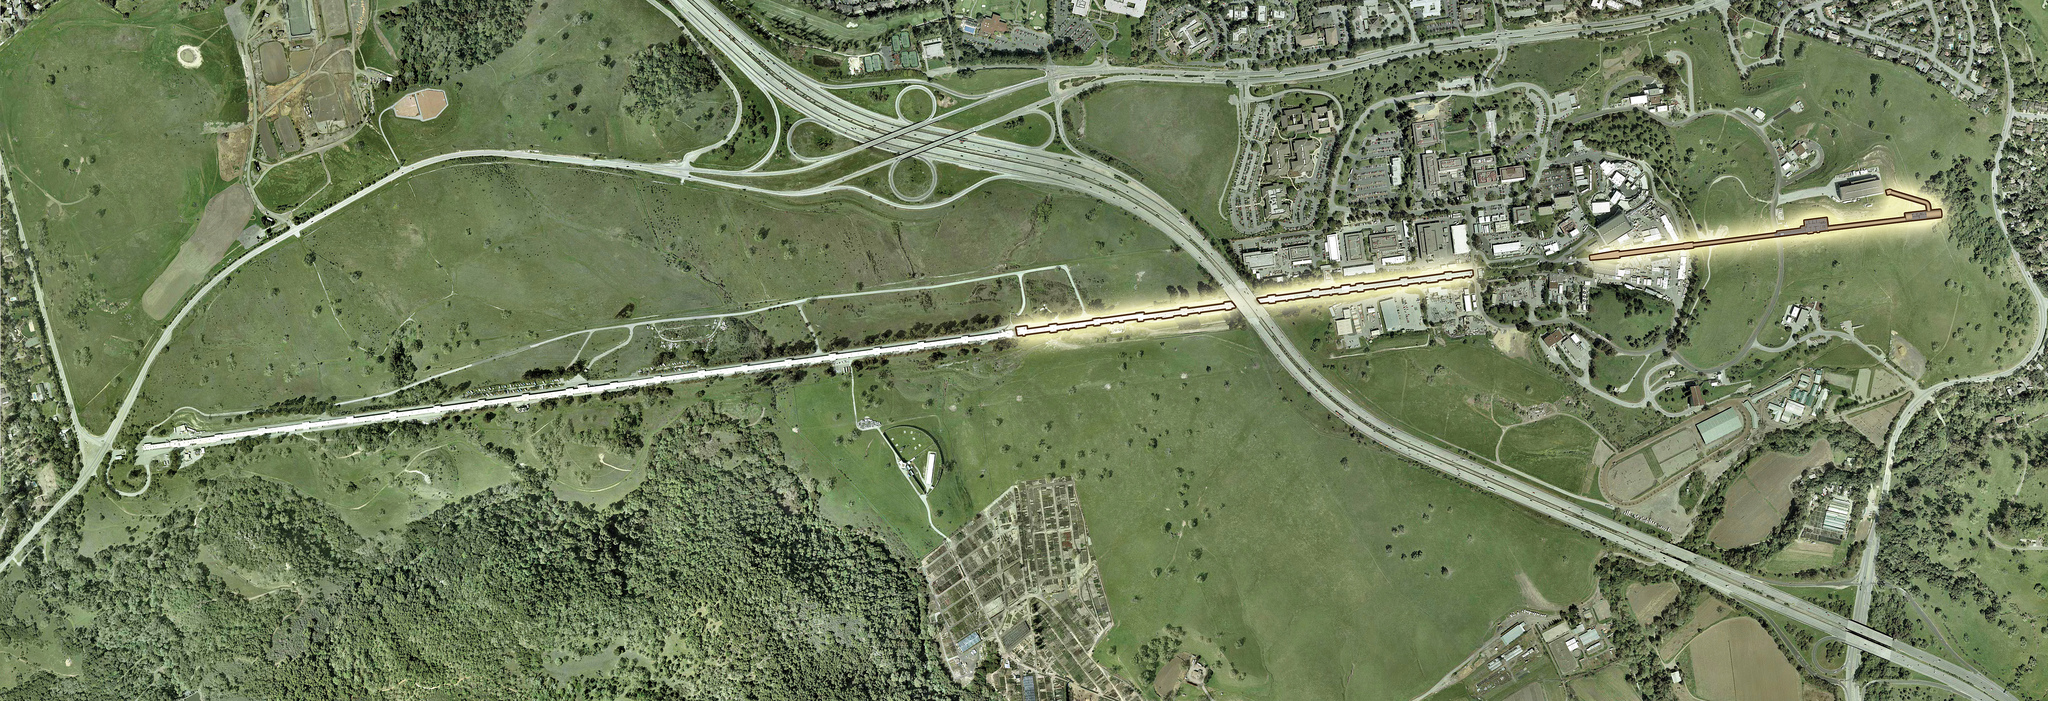
\includegraphics[width=1.00\textwidth]{images/aerial-view-lcls.jpg}
	\caption[Aerial view of the Linac Coherent Light Source.]{Aerial view of the Linac Coherent Light Source\index{Linac Coherent Light Source}. LCLS\index{LCLS|seealso {Linac Coherent Light Source}} uses the last third of SLAC's linear accelerator but is overall a multikilometer long machine. The accelerator and buildings are stretched far because of the light generation process. From \citep{SLAC-2009-Flickr}}
	\label{fig:aerial-view-lcls}
\end{figure}
To get a numerical understanding, let us look at sequential photon absorption dynamics in atoms and molecules. One can conservatively estimate that a typical absorption cross section for soft X-rays\footnote{Soft X-rays have wavelengths of \SIrange{10}{\sim 0.2}{\nano\meter}} is around $\sigma = 1$ megabarn (Mb) \citep{Bucksbaum-2011-Book}. Typical X-ray foci\footnote{The focus size at the AMO instrument of LCLS is $\SI{1}{\micro\meter\squared}$.} are $A = \SI{1}{\micro\meter\squared}$ such that the number of photons, $n_{in}$, needed to absorb just one photon per atom, $n_{abs}$, is
\begin{equation}
n_{in} = \frac{n_{abs} A}{\sigma} = \frac{10^{-8}}{10^{-18}}\si[per-mode = fraction]{\cancel\square\centi\meter\per\cancel\square\centi\meter}=10^{10}\qquad \mathrm{photons.}
\label{eq:absorption-cross-section}
\end{equation}
We can compare this to a modern synchrotron source, for example, the Advanced Photon Source at Argonne National Laboratory. This synchrotron facility produces \num{\sim e6} photons per pulse in the Si(111) bandwidth at pulse durations of a few tens of picoseconds \cite{Young-2017-PC}. That is far out of reach for investigating non-linear, or multi-photon, processes. While this back of the envelope type of calculation might be off by an order of magnitude or so depending on the specific case, it illustrates the orders of magnitude increase in the number of photons scientists were looking for to unravel entirely new aspects of X-ray science. As it is not possible to use conventional optical methods to increase the number of X-ray photons, drastic ideas were needed. Reference \citep{Madey-1971-JAP} described in the 1970's the idea of coherent radiation in the ultraviolet to X-ray region, and over ten years later, the construction of free electron lasers was proposed \citep{Kondratenko-1980-PA,Bonifacio-1984-OC}. The Section \ref{sec:sase} discusses the laser-like radiation in the X-ray region of these light sources in more detail.\\[1\baselineskip]
%
%Free electron lasers, amplify the light along a straight line to create laser-like radiation. 
Construction of the first hard XFEL, the Linac Coherent Light Source\index{Linac Coherent Light Source}, finished in 2009. Figure \ref{fig:aerial-view-lcls} shows LCLS from a birds-eye view. LCLS is able to create \num{\sim e12} photons per pulse and achieves pulse-lengths of a few femtoseconds. The beam parameters of XFELs increased the peak brightness that is available at user facilities by many orders of magnitude\footnote{See Figure \ref{fig:soft-xray-self-seeding} for an illustration of the improvement in peak brightness.}. This allows the study of, for example, the above mentioned sequential absorption of photons in atoms and molecules \cite{Young-2010-Nature,Berrah-2011-PNAS}, non-linear dynamics of atoms \cite{Rohringer-2012-Nature}, the ultrafast movement of electrons in chemical reactions \cite{Dell-Angela-2013-Science,Picon-2016-NatComm,Rudenko-2017-Nature}, and the imaging of nanoparticles \cite{Seibert-2011-Nature,Gorkhover-2012-PRL}.\\[1\baselineskip]
%
Only a few XFELs exist today. The LCLS at SLAC National Accelerator Laboratory (SLAC) in the United States and the SACLA at Rikagaku Kenkyūsho (RIKEN) in Japan are the two currently operating XFEL user-facilities. More XFELs are being built around the world, for example, the European XFEL near Deutsches Elektron Synchrotron (DESY) in Germany, the SwissFEL at Paul Scherrer Institut (PSI) in Switzerland, and the PAL-XFEL at Pohang Accelerator Laboratory (PAL) in South Korea.
%
%
%
\subsection{From bending magnets to undulators}\label{sec:undulator}
%%%%%%%%%
%- Idea and schematic setup\\
%- Explain SASE including micro-bunching\\
%- Talk about the importance of monitoring the energy loss
%%%%%%%%%
\begin{figure}[t]
	\centering
	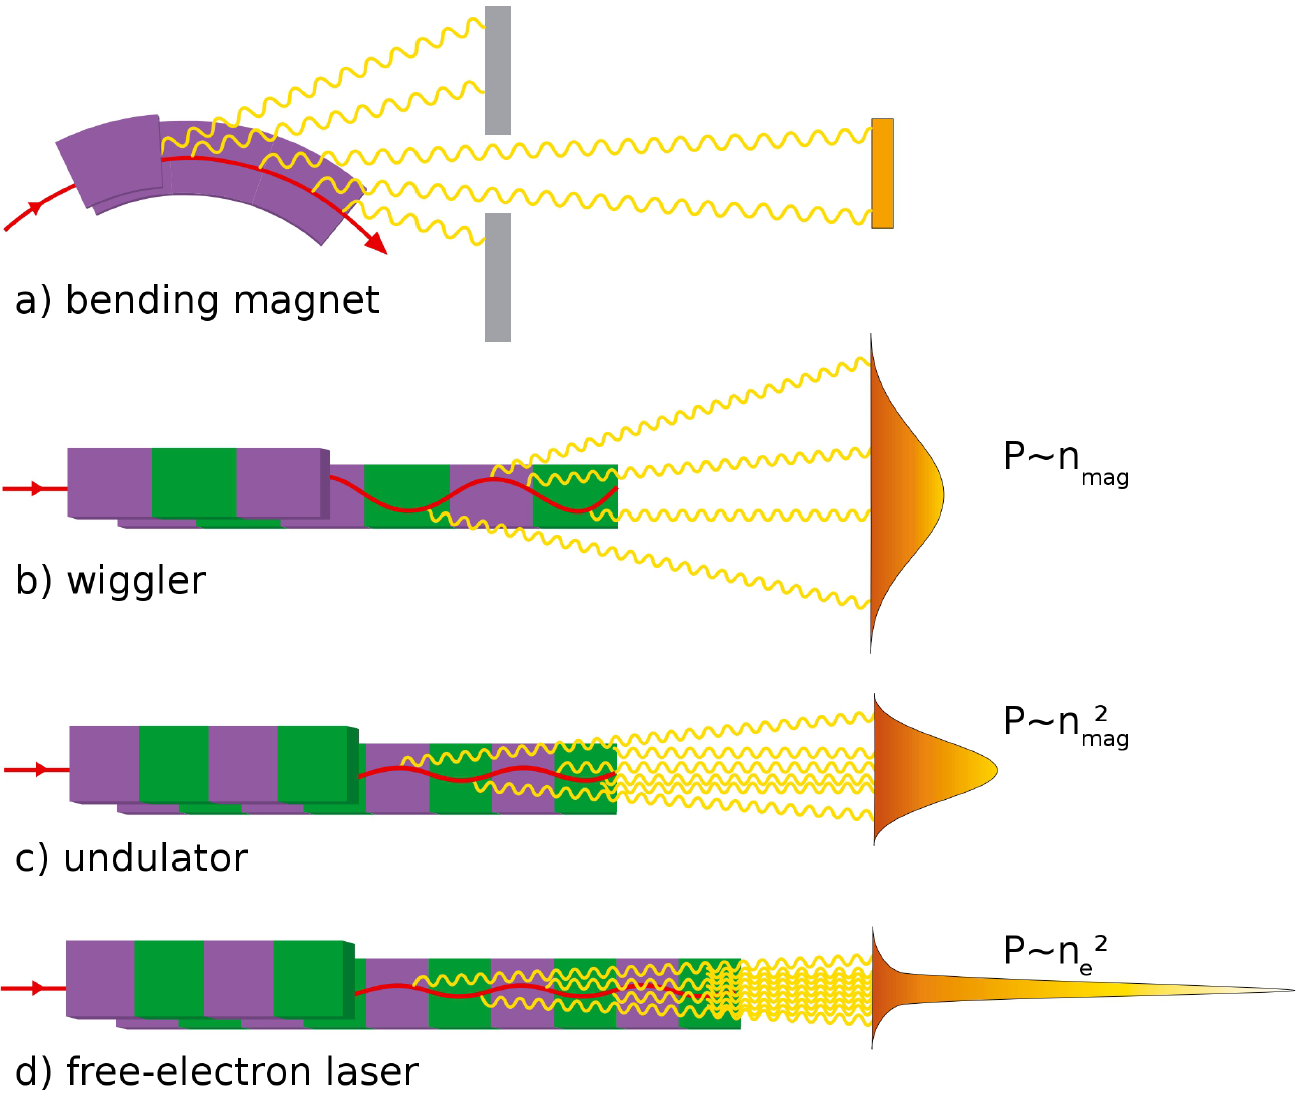
\includegraphics[width=0.70\textwidth]{images/bending-to-FEL.png}
	\caption[Schematics of several X-ray generating methods.]{Schematics of several X-ray generating methods using magnets (purple \& green). The red lines are pathways of the electron beams and the yellow lines represent emitted X-rays. The emitted spatial power distribution is orange. From \citep[\href{http://creativecommons.org/licenses/by-nc-nd/3.0/de/}{\ccbyncndeu}]{Rupp-2013-Thesis}.}
		%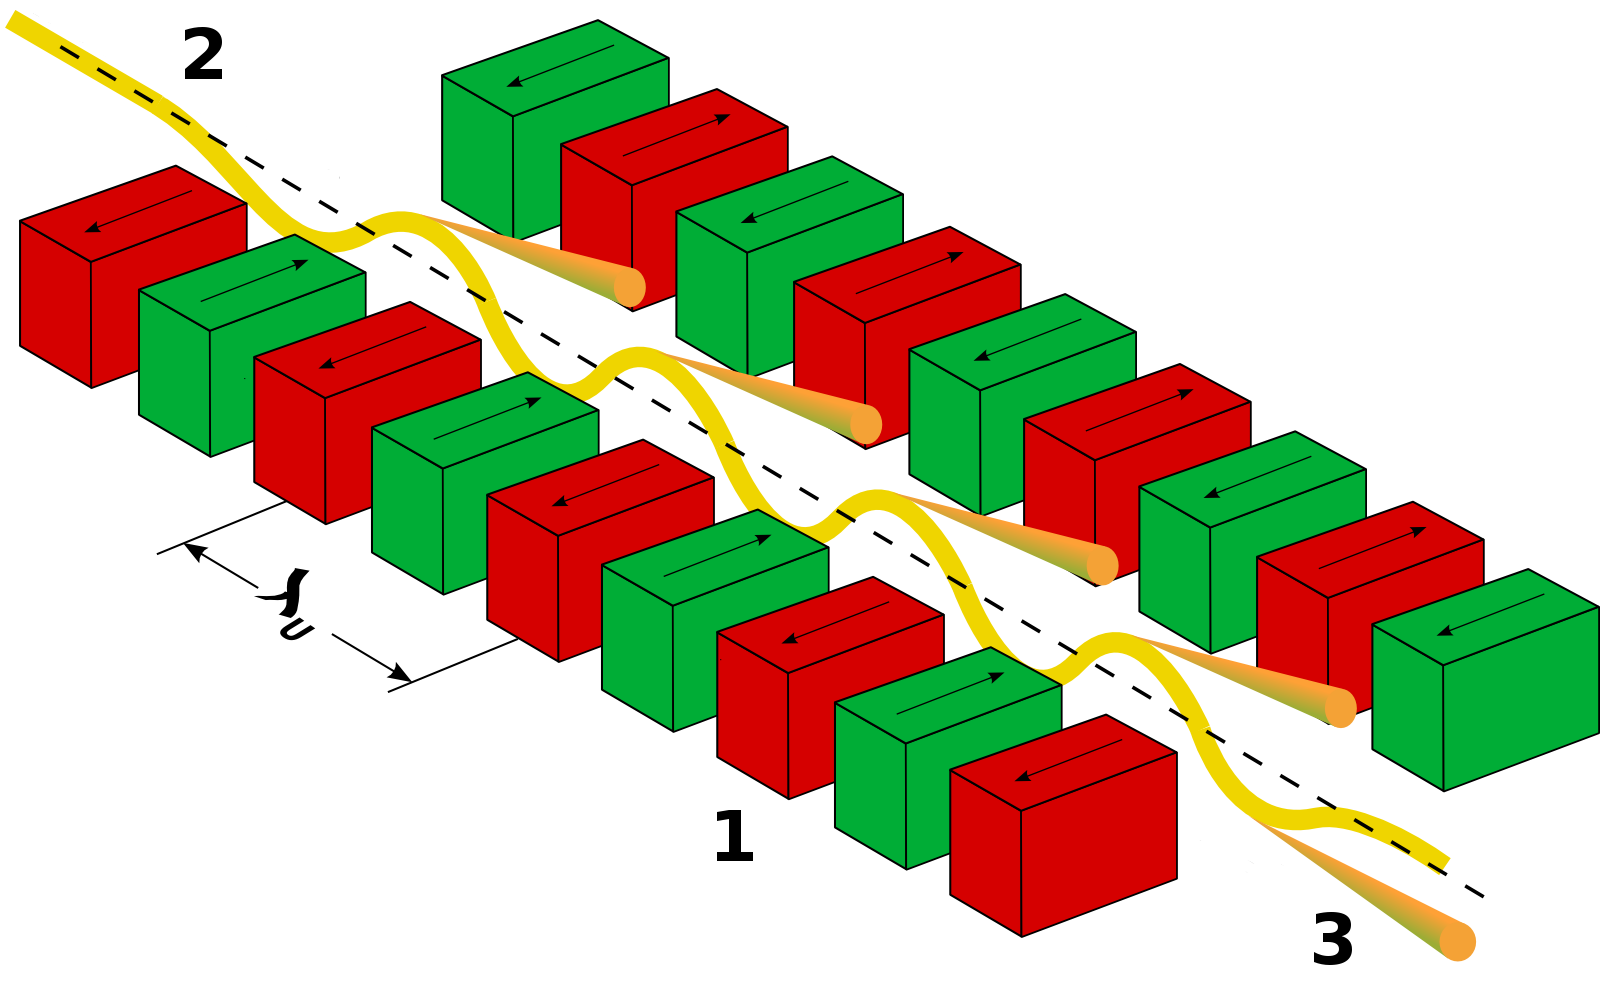
\includegraphics[width=1.00\textwidth]{images/Undulator.png}
	%\caption[Schematic setup of an undulator.]{Schematic setup of an undulator with a period of $\lambda_{U}$. (1) Magnets in alternating polarity; the arrows indicate the direction of the magnetic field. (2) Incoming electron bunch near the speed of light. (3) Emitted light in beam direction due to sinusodial movement of the electron bunch. From \citep{holst-2005-wiki}.}
	\label{fig:undulator}
\end{figure}
In the initial X-ray synchrotron light sources\index{light source}, the radiation was generated using \textit{bending magnets}\index{bending magnets} as explained earlier in Section \ref{sec:xfel}. A schematic setup of a bending magnet can be seen in Figure \ref{fig:undulator}. The first improvement to creating X-rays over bending magnet sources was through a \textit{wiggler}\index{wiggler}. Wigglers consist of magnets arranged in an alternating polarity. An electron bunch traveling through a wiggler is ``wiggled'' along its path due to magnetic fields, which causes the particles to emit radiation. Wigglers can be considered as a series of bending magnets, which is why the total emitted power, P, is proportional to the number of magnets, n$_{\text{mag}}$, \citep{Brown-1983-NIMPR}
\begin{equation}
\text{P} \propto \text{n}_{\text{mag}},\quad \text{in a wiggler magnet.}
\end{equation}
The emitted radiation has a broad, continuous spectrum and the center of that spectrum can be controlled by changing the speed, or kinetic energy, of the electron bunch. For X-rays, wigglers were first used by the Hamburger Synchrotronstrahlungslabor (HASYLAB) at DESY and the Stanford Synchrotron Radiation Light-source (SSRL) at SLAC in the late 1970's to early 80's. Independently from wigglers, undulators\index{undulator} were developed \citep{Williams-2009-xb}. Wigglers and undulators create radiation on the same principle: an electron bunch is accelerated near the speed of light and then forced on a sinusoidal pathway. 
%In undulators, the separation of magnets is specific and named undulator period, $\lambda_{U}$. 
Although wigglers and undulators are large constructs of a few meters and their magnet spacing is on the order of centimeters, traversing electrons can emit radiation on the nanometer wavelength range. This is due to relativistic effects. In the frame of the electrons, the magnet spacing appears shorter. Wigglers and undulators can be characterized by the strength parameter, $K$, which is given by \citep{Huang-2007-PRSTAB}
\begin{align}
K &= \frac{e\ B_{\text{max}}\ \lambda_{U}}{2 \pi\ m_{e}\ c},
\intertext{where $e$ is the elementary charge, $B_{\text{max}}$ is the maximum magnetic field in the undulator or wiggler, $m_{e}$ is the mass of an electron, $c$ is the speed of light, and $\lambda_{U}$ is the so-called \textit{undulator period} that corresponds to the magnet spacing. $K$ can be expressed in convenient units}
K &\approx 0.934\ B_{\text{max}}\ \lambda_{U}\qquad \left[\si{\tesla\centi\meter}\right],
\label{eqn:undulator-strength}
\end{align}
and wigglers typically have $K\gg \SI{1}{\tesla\centi\meter}$, while undulators usually have $K < \SI{1}{\tesla\centi\meter}$. The X-rays emitted by undulators typically have a narrower spectrum and a higher flux than wigglers. This is due to the fact that the undulator period and magnetic fields are chosen specifically in an undulator. The parameters are set such that their emitted radiation per period constructively interferes with each other. This resonance condition is expressed by the \textit{fundamental wavelength} of an undulator, $\lambda_{r}$, and can be noted as \citep{Huang-2007-PRSTAB}
\begin{equation}
\lambda_{r} = \frac{\lambda_{U}}{2 \gamma}\left(1+\frac{K^{2}}{2}+\gamma^{2}\Psi^{2}\right),\label{eqn:fundamental-wavelength}
\end{equation}
with the Lorentz factor $\gamma$ of the electron bunch in the undulator and the electron observation angle, $\Psi$. As a result, the emitted power, P, now scales as \citep{Kim-1986-NIMPRA}
\begin{equation}
\text{P} \propto \text{n}_{\text{mag}}^{2},\quad \text{in an undulator magnet.}
\end{equation}
%Summarizing, modern lightsources use undulators to generate radiation as these magnets create more photons that have a narrow spectral bandwidth compared to bending magnets and wiggler. Undulators are characterized by the strength parameter given in Equation \eqref{eqn:undulator-strength}, which is only dependent on the undulator gap $\lambda_{U}$ and the magnetic field $B$. The fundamental amplified wavelength is given by the resonance condition Equation \eqref{eqn:fundamental-wavelength}.\\
%
%
%
\subsection{Self-amplification by spontaneous emission}\label{sec:sase}
\begin{figure}
	\centering
		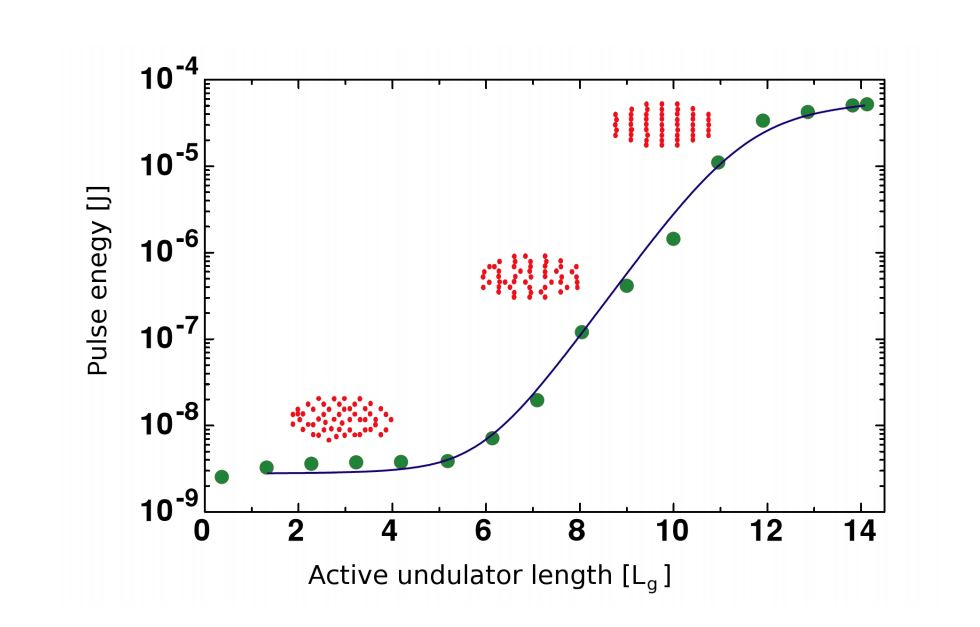
\includegraphics[width=0.7\textwidth]{images/gain-length.JPG}
	\caption[Undulator gain curve correlated to microbunching.]{Undulator gain curve correlated to microbunching. The X-ray pulse energy is plotted logarithmically over the undulator length $L_{g}$ (blue curve, green dots) and shows an exponential growth until saturation. The electron bunch (red dots) starts with a random density distribution. As the bunch travels through the undulator, its density is periodically modulated such that the electrons microbunch. Upon optimal \textit{microbunching}, the X-ray lasing process saturates. From \citep{Rupp-2013-Thesis,Rupp-2016-Springer}}
	\label{fig:gain-length}
\end{figure}
If an electron bunch travels through just one undulator, the emitted power scales linearly with the number of electrons, n$_{\text{e}}$, which is due to the finite size and randomly distributed density of an electron bunch. If the electrons emit light from the same point or are separated by $i\cdot \lambda_{r}$, with $i=\left(1, 2, 3, ...\right)$, the emitted photons would constructively interfere and be coherent \cite{Als-Nielson-2011-JWS}. This idea - to emit light from a point-like source - is exploited in XFELs by \textit{microbunching}\index{microbunching} the electron bunches. Simplified this means that electrons of a bunch are microscopically structured to stripes, which is illustrated in Figure \ref{fig:gain-length}. Following the figure, microbunching can be created in a straight and long undulator section\footnote{LCLS has a \SI{112}{\meter} long undulator section.}, where multiple undulators are connected in series. As the electron bunch travels in vacuum through the long XFEL undulator section, light is faster than the electrons. This slight velocity difference means that the co-propagating photons and electrons have a phase difference and interact with each other. Depending on the phase, an electron will either gain or lose velocity. As a result, the initial uniform electron density is periodically modulated by the photon-field as it travels through the undulators of an XFEL \cite{Huang-2007-PRSTAB}. The modulated electron bunch structure is called microbunching.\\[1\baselineskip]
%
The key process in microbunching is that an electron bunch interacts with the emitted photon-field. The interaction occurs only because the particles have a narrow spatial and kinetic-energy distribution. The average spread of these distributions can be characterized by the so-called \textit{emittance}\index{emittance}. And only the linear accelerator components of a free electron laser (FEL) are able to compress an electron bunch in space and energy, i.e., create a low-emittance electron-bunch such that the electron bunch can interact with the photons and microbunch.\\[1\baselineskip]
%
At LCLS, the low-emittance attribute effectively reduces the Equation \ref{eqn:fundamental-wavelength} to $\lambda_{r}(\Psi \rightarrow 0)$ \cite{Bucksbaum-2011-Book}. This allows us to further describe the structure of the microbunching. Due to the velocity mismatch of the electrons and the photons, the photon-field travels the distance $\lambda_{r}(\Psi = 0)$ more than the electron bunch over each undulator period, $\lambda_{U}$. This distance is also referred to as \textit{slippage} and affects the modulation period of the electron density as mentioned above. The spacing between the dense areas is therefore $\lambda_{r}(\Psi = 0)$ (see Figure \ref{fig:gain-length}). As the electron bunch becomes structured, it amplifies a narrower wavelength bandwidth around $\lambda_{r}(\Psi = 0)$ through spontaneous emission. As more photons travel along-side the electron bunch, the bunch becomes even more structured and one speaks therefore of ``self-amplification''. Eventually the microbunching is fully developed and the lasing process saturates.\\[1\baselineskip]
%
This type of radiation, or XFEL operation mode, is called \textit{Self-Amplification by Spontaneous Emission} (SASE) above described processes. The emitted power, P, is now not only proportional to the square of the number of undulator magnets but due to the point-like emission it also scales as \citep{Als-Nielson-2011-JWS}
\begin{equation}
\text{P} \propto \text{n}_{\text{e}}^{2},\quad \text{in SASE operation.}
\end{equation}
Single-shot and average SASE spectra can be seen in Figure \ref{fig:SASE-spectra}. A SASE spectrum is typically different from shot-to-shot and has distinct peaks on top of a more broad background. This is due to the initially emitted photons that have a pseudo-random wavelength within a narrow bandwidth. The electron-bunch amplifies these specific wavelengths as it travels through the undulators since its microbunching is defined by those specific wavelengths.\\[1\baselineskip]
%Initially (random) created photons in the undulator define the microbunching as it travels through the undulators and amplifies these photons through subsequent spontaneous emission.
\begin{figure}
	\centering
		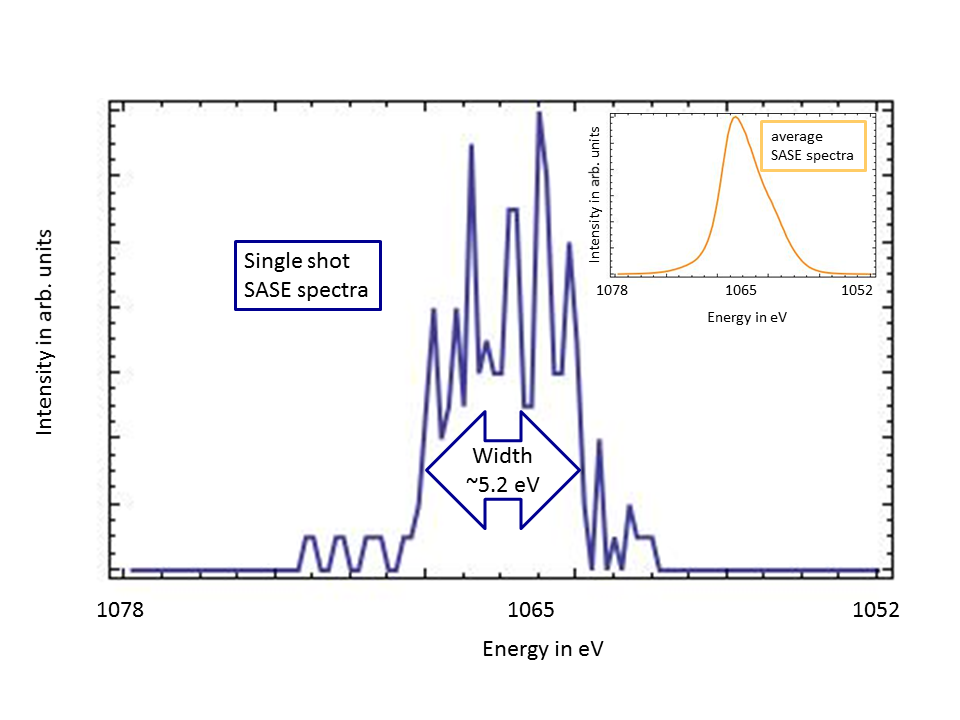
\includegraphics[width=0.65\textwidth]{images/SASE-spectra.png}
	\caption[SASE single-shot and average spectra.]{The large blue spectra is a SASE spectra from a single LCLS shot measured with a hemispherical analyzer \citep{Bucher-2014-Unpublished}. Note the spiky peak structure on a background pedestal. Within the narrow bandwidth of an XFEL pulse some energies are more strongly amplified due to the microbunching. The yellow graph in the inset is an average spectrum of several hundred single-shots and shows a low energy tail, which is due to XFEL-jitter.}
	\label{fig:SASE-spectra}
\end{figure}
%
There are different types of FEL that can produce SASE radiation. Typically at longer wavelength ranges, where efficient optics are readily available, a so-called \textit{multi-pass low-gain} FEL is able to reuse electron-bunches, despite the fact that the lasing process affects the kinetic energy of the bunch. Without going into much detail, this FEL type leads to comparable high repetition rates and narrow spectra but few photons per pulse \citep{Kim-2008-PRL}. At shorter wavelength ranges, the kinetic energy of an electron bunch is drastically affected due to the X-ray lasing process. Additionally, there is a lack of efficient optics in the X-ray region. So, XFELs use only one electron-bunch\footnote{The European XFEL uses a so-called \textit{bunch train}, where multiple electron bunches are accelerated in series.}, which is \textit{dumped} after a long undulator section. This is called a \textit{single-pass high-gain} FEL.
%
%
%
%
\subsection{Soft X-ray self-seeding}\label{sec:sxrss}
%%%%%%%%%%%%%%%%%%%%%%
%- Should I include this section? I could use it for the pump probe as well\\
%- Self seeding vs. seeded FELs\\
%- Schematic setup of a self seeding unit\\
%- Work towards self-seeded beams including spectrometer data
%%%%%%%%%%%%%%%%%%%%%%
%
\begin{figure}
	\centering
		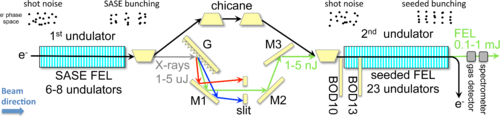
\includegraphics[width=0.90\textwidth]{images/seeded.png}
	\caption[Schematic setup of soft X-ray self-seeding system.]{Schematic setup of the soft X-ray self-seeding system at LCLS. The X-rays are reflected of grating (G) and mirrors (M1-M3) and act as seed when they are overlapped with the electron bunch again using the beam overlap diagnostics (BOD10 \& BOD13). From \citep{Ratner-2015-PRL}. Reprinted with permission from APS.}
	\label{fig:seeded-setup}
\end{figure}
%
A special free electron laser beam mode is the seeded type. In contrast to the SASE operation, where the initial photons are randomly emitted and further amplified, a seeded FEL starts with a given \textit{seed} of photons. If the set of initial photons is monochromatic, mostly this wavelength is amplified as the bunch travels through the undulator along-side the seed. The initial photon seed can be created through various processes and the wavelength of the photon seed is the critical parameter in determining which method to choose. In the case of the infra-red (IR) to extreme ultra-violet (XUV) wavelength range, conventional lasers can be used to produce the initial photon seed. However, due to the lack of lasers available at X-ray wavelengths, the idea of \textit{self-seeding}\index{self-seeding} is pursued.\\[1\baselineskip]
%
\begin{figure}
	\centering
		a)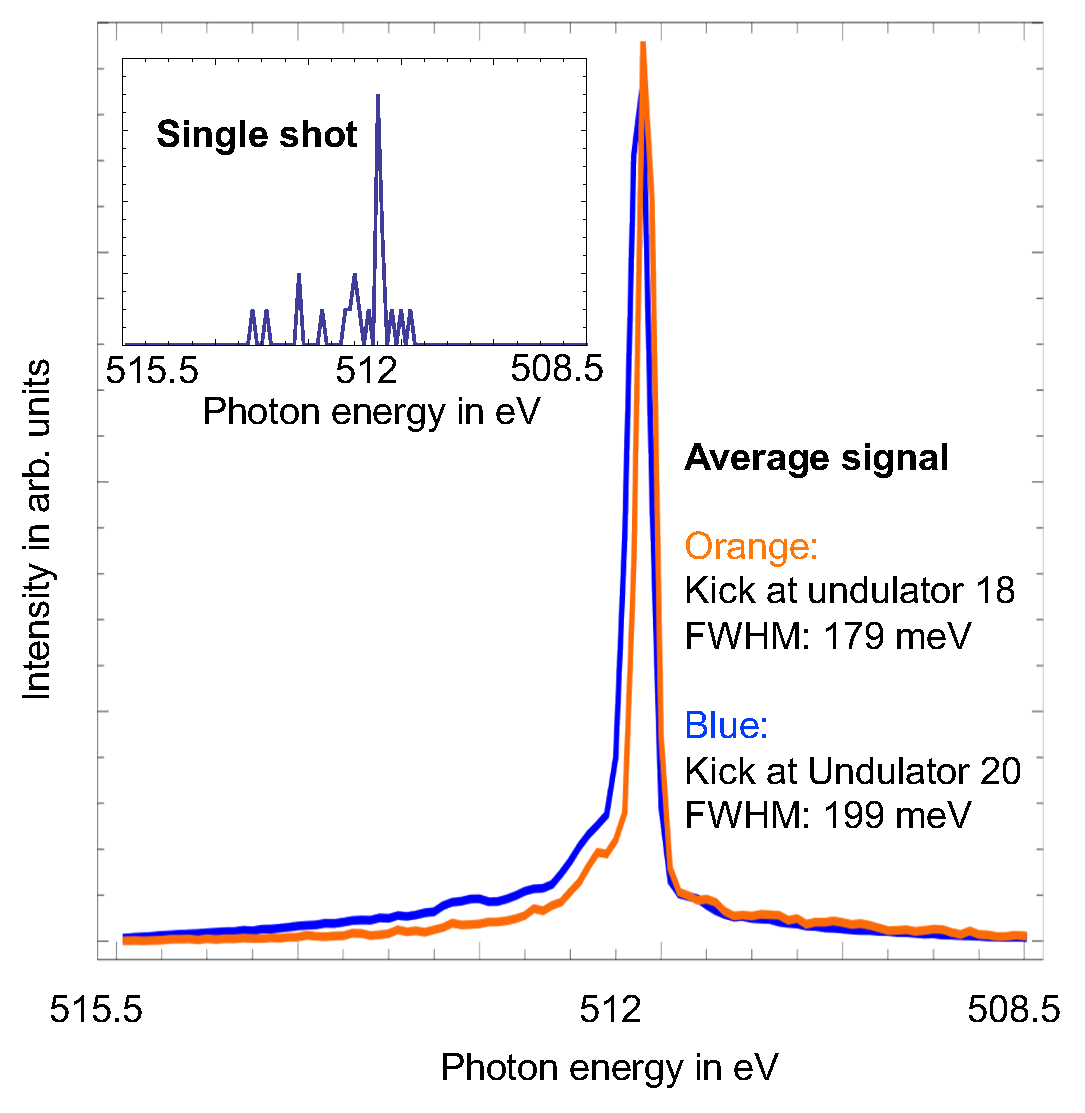
\includegraphics[width=0.40\textwidth]{images/Soft-X-ray-self-seeding.pdf}
		b)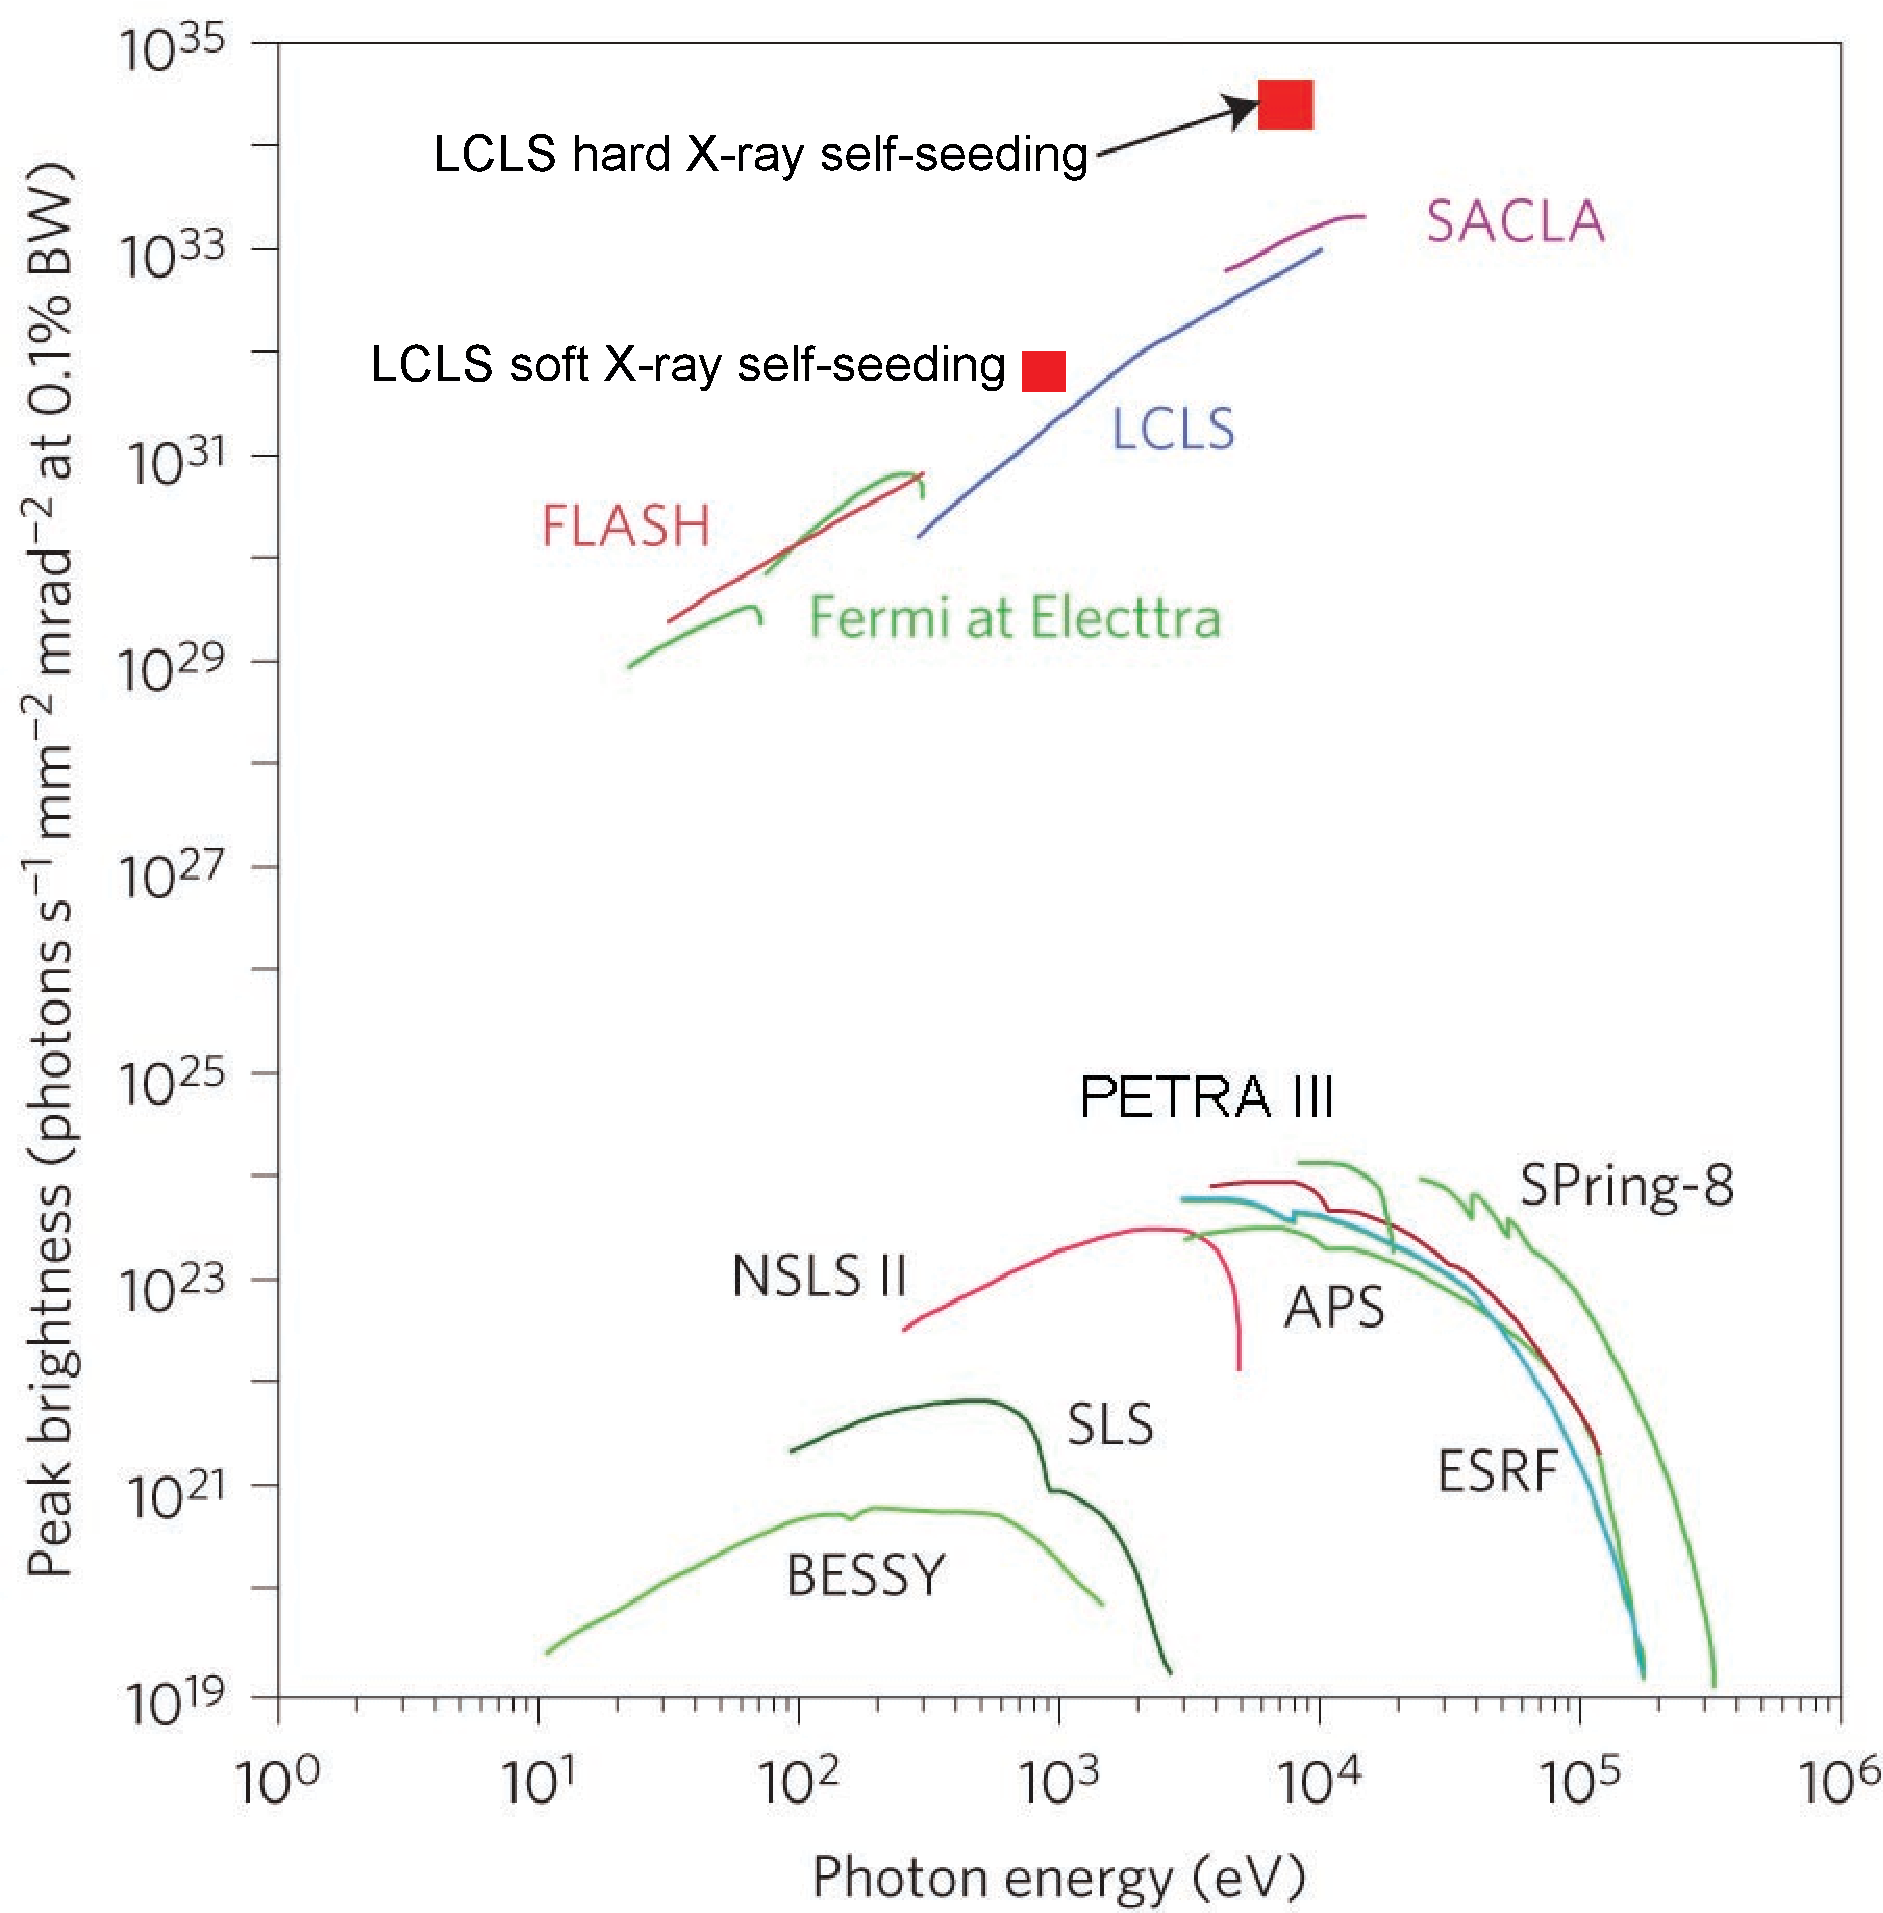
\includegraphics[width=0.40\textwidth]{images/spectral-brightness-fletcher-2015-corr2.pdf}
	\caption[Soft X-ray self-seeding spectra and brilliance of various light sources.]{a) Normalized average spectra of soft X-ray self-seeding operations using the AMO instrument at LCLS. The self-seeding spectra is characterized by a sharp spectral peak around the seed energy, which is accompanied by a SASE pedestal. The often undesired pedestal is suppressed when the undulators length is shortened \cite{Bucher-2014-Unpublished}. b) The peak brightness of various light sources over a wide photon energy range. Self-seeding operations have a higher peak brightness than current SASE operations. Adapted from \cite{Fletcher-2015-NatPho,Ratner-2015-PRL}.}
	\label{fig:soft-xray-self-seeding}
\end{figure}
%
Following Figure \ref{fig:seeded-setup}, an electron bunch is first sent through a few undulator magnets to generate a few SASE photons. The electrons and photons are then separated using a magnetic chicane, which also neutralizes the microbunching in the electron bunch. The grating monochromator selects a small wavelength slice from the comparably broad SASE spectrum of the initial photons. Photons exiting the monochromator are called the \textit{seed}. The seed and the electron bunch are overlapped again using the magnetic chicane and then sent through more undulators. Here, the seed modulates the electron bunch and thus only a narrow spectral band is amplified. A typical spectrum of a soft X-ray self-seeded beam can be seen in the left panel of Figure \ref{fig:soft-xray-self-seeding}. The characteristics of a self-seeded spectrum are an intense peak at the wavelength of the seed on top of a broad SASE background pedestal. The background is an artifact of the amplification of some spontaneous emission events and can be suppressed by using fewer undulator magnets. Self-seeded beams have a significantly reduced pulse energy -- by an order of magnitude or so, depending on the exact beam parameters -- as compared to LCLS SASE operations. However, in their main peak, self-seeded pulses have a higher spectral peak brightness when compared to SASE pulses. Using Equation \eqref{eq:spectral-brightness}, the increase in spectral brightness compared to SASE is understandable due to reduced bandwidth. The increase in peak brightness is illustrated in the right panel of Figure \ref{fig:soft-xray-self-seeding} and compared to other modern X-ray light sources.\\[1\baselineskip]
%
Self-seeded beam operations have recently been demonstrated at LCLS. For hard X-rays, the Hard X-Ray Self-Seeding (HXRSS) instrument uses a diamond crystal to select a wavelength slice \citep{Amann-2012-NatPho}. In the case of soft X-rays, the Soft X-ray Self Seeding (SXRSS)\index{self-seeding!soft x-ray} instrument uses a grating monochromator \citep{Ratner-2015-PRL}. A seeded beam using an external laser to generate photons as an initial seed has been demonstrated at the XUV-FEL FERMI at Ellettra-Sincrotrone (ELETTRA) in Italy \citep{Allaria-2012-NatPho}. The peak intensity in a narrow spectral band makes seeded beams interesting for a variety of applications, particularly in spectroscopy, where it is momentous to excite materials with narrow bandwidth photons. There are also applications in atomic and molecular physics, ranging from absorption spectroscopy \citep{Ferguson-2014-Unpublished}, to ultrafast photoelectron spectroscopy on molecules \citep{Bucher-2014-Unpublished}, and to non-linear stimulated Raman spectroscopy \citep{Kimberg-2016-FD}. Particularly interesting for this work is the magnetic chicane from the SXRSS instrument when used as described in the next section.
%
%
%
%
\subsection{Novel X-ray pump–X-ray probe techniques}\label{sec:novel-pump--probe-tech}
%%%%%%%%%%%%%%%%%
%- Albertos pump-probe version\\
%- Agos two color pump probe version\\
%- Ratners and Agos seeded pump probe version\\
%- Use spectra from single-shot spectrometer
%%%%%%%%%%%%%%%%%%%%%%%%
Pump--probe experiments are commonly used as they allow a precise study of dynamics. The pump-pulse gives a very controllable starting point, i.e., ``time zero'' in the dynamic process, and the probe-pulse can perform a measurement of the dynamics at a later time delay, $\Delta t$. Sometimes pump- and probe-pulse are switched, which is indicated by negative time delays and used to verify time zero, or to probe the system before any dynamics have occurred.
It is often desirable to have a pump- and probe-pulse of different wavelength, for example, one can pair an optical laser pulse and an X-ray pulse.
%, or XFEL can produce two X-ray pulses of different wavelength, which are called ``two-color'' pump--probe schemes.
However, in order to study X-ray induced phenomena using X-ray imaging and spectroscopy techniques, as discussed in this thesis, two X-ray pulses are needed.\\[1\baselineskip]
%
Recently, two methods have been proposed to create two X-ray pulses to conduct a X-ray pump--X-ray probe experiment. Method one is a mirror-based beam split-and-delay system (XRSD device) \citep{Castagna-2013-JPCS,Murphy-2012-SPIE,Berrah-2016-OE}. It splits a single pulse into a pump- and probe-pulse, allowing a time delay of the latter. These systems are typically limited to short time delays, as the grazing incidence optics have to fit into existing setups. Method two uses accelerator-based schemes \citep{Lutman-2013-PRL,Marinelli-2015-NatComm} that manipulate electron bunches to create two X-ray pulses.
%Limitations arise depending on the scheme, e.g., limited pulse delay, $\Delta t$, or pulse energy split through limited electron beam separation or length of magnetic chicane.
Both methods have been demonstrated at LCLS and have been complementing the more widely available optical laser pump--X-ray probe methods, particularly in the chemical sciences \citep{Picon-2016-NatComm,Ferguson-2016-SciAdv,Liekhus-Schmaltz-2015-NatComm}.\\[1\baselineskip]
%
The accelerator-based X-ray pump--X-ray probe method used in this thesis can also produce two X-ray pulses of different wavelength, which are so-called ``two-color'' pump--probe schemes. The generation of two-colored X-ray pulses is based on the parameters of Equation \eqref{eqn:fundamental-wavelength} and indicates two possible schemes: one, the undulator parameter, $K$, can be tuned to change the emitted wavelength; and two, the Lorentz factor, $\gamma$, can be different if there are two electron bunches. As the accelerator-based X-ray pump--X-ray probe method has been used in the present work, let us describe these schemes in greater detail.
%
%
%
\subsubsection{Undulator parameter-$K$ based pump--probe schemes}\label{sec:k-based-pump--probe}
%
\begin{figure}
	\centering
		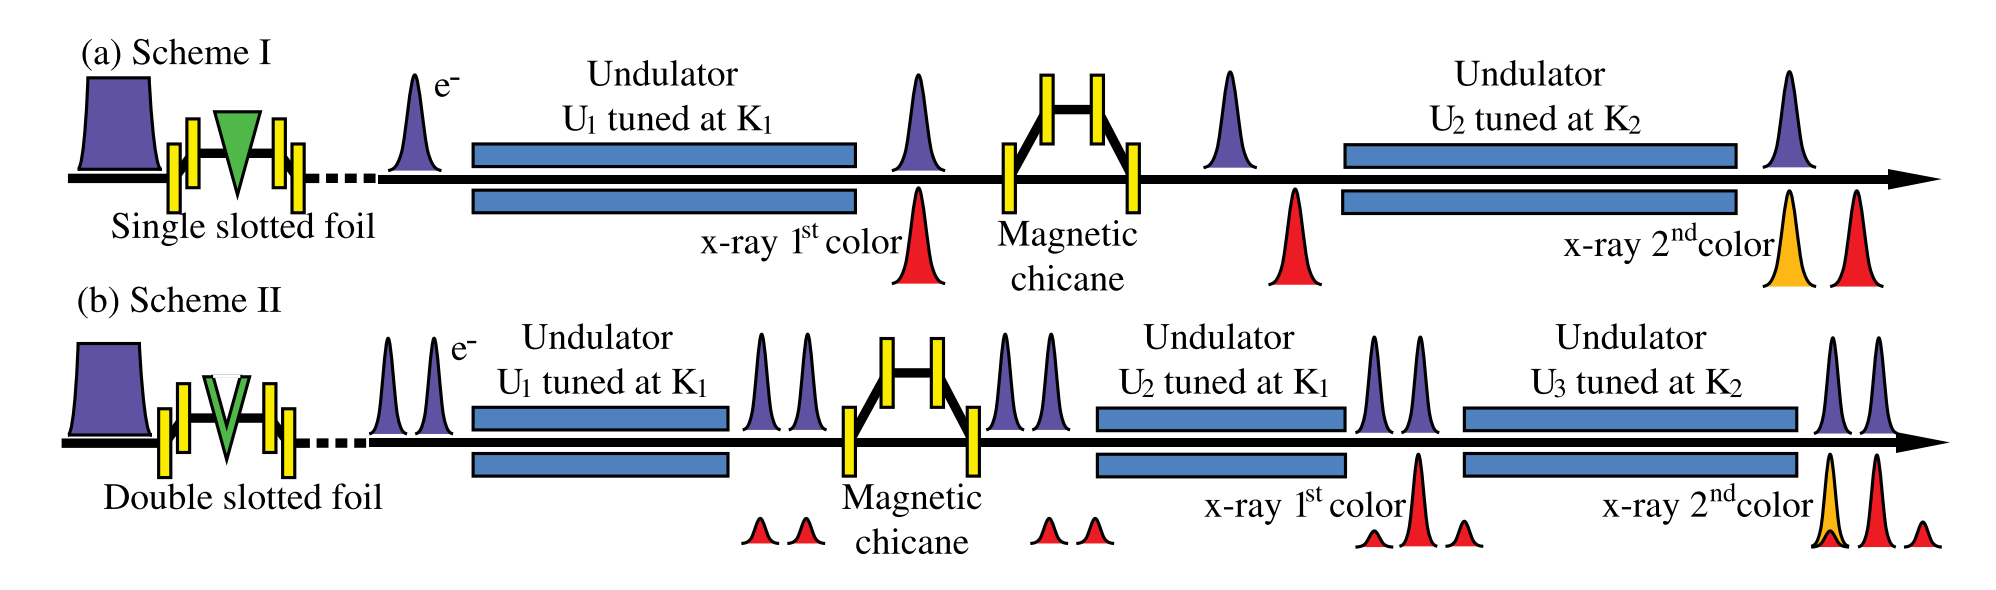
\includegraphics[width=1.00\textwidth]{images/Albertos-pump-probe-scheme.png}
	\caption[Schematic setup of an undulator based pump--probe scheme.]{Schematic setup of undulator parameter-K based pump--probe schemes at LCLS. In (a) Scheme I, one creates a single electron bunch using a single slotted foil. (b) Scheme II, one creates a double electron bunch using a double slotted foil. The electron bunches emit radiation with a wavelength depending on K$_{1,2}$. A time delay $\Delta t$ between pulses is introduced using a magnetic chicane. From \citep{Lutman-2013-PRL}. Reprinted with permission from APS.}
	\label{fig:Albertos-pump-probe-scheme}
\end{figure}
%
The first developed accelerator based X-ray pump--X-ray probe technique at LCLS \citep{Lutman-2013-PRL} uses a difference in undulator parameters, $K_{1,2}$, to create two pulses of different wavelength. The time delay is introduced through a magnetic chicane.\\[1\baselineskip]
%
A schematic setup is shown in Figure \ref{fig:Albertos-pump-probe-scheme}.
Following the figure in the top panel (a) Scheme I, one electron bunch is created through a single slotted foil\footnote{A single slotted foil or emittance-spoiling foil is typically inserted in a magnetic chicane. Here, it spoils the electron bunch by Coulomb scattering them leaving only a certain energy band of the electron bunch that is within the slot unspoiled. This usually narrows the electron beam and thus reduces its pulse duration \citep{Emma-2004-PRL}.}. The use of the slotted foil enables control over the pulse duration. The electron bunch then travels through the undulator section $U_{1}$ tuned at strength parameter $K_{1}$ and is stimulated deep into the lasing process, but the lasing does not go into saturation such that the electron bunch can be reused in the second undulator section. A magnetic chicane removes the microbunching from the section $U_{1}$ such that in undulator section $U_{2}$, tuned to undulator strength parameter $K_{2}$, the electron bunch lases again and the process is able to saturate. The maximal color separation between the two pulses is \SI{\sim 1.9}{\percent} in relative difference between $K_{1}$ and $K_{2}$.\\[1\baselineskip]
%
The time delay between the two pulses is introduced by a magnetic chicane that extends the pathway of the electrons and leaves photons unaffected. At LCLS, a dedicated chicane, for example, from the soft X-ray self-seeding instrument (see Section \ref{sec:sxrss}), can reach delays up to a maximum of $\SI{800}{\femto\second}$.
In this scheme, several factors prevent a minimal time delay, $\Delta t_{\text{min}}$, of zero. The minimal time delay opposed by the magnetic chicane, $\tau_{\text{min}}$, is dictated by the electron drift velocity mismatch to the speed of light. We can express that as,
\begin{equation}
\tau_{\text{min}} = \frac{l}{v_{\text{drift}}} - \frac{l}{c}\approx \SI{50}{\atto\second},
\label{eq:alberto-delta-t-min}
\end{equation}
with $l\approx \SI{4}{\meter}$ being the length between undulator sections $U_{1}$ and $U_{2}$, $c$ being the speed of light, and $v_{\text{drift}}$ being the drift velocity of the electron bunch. As the electron bunch drifts undeflected through the chicane close to the speed of light $\tau_{\text{min}}$ is typically on the tens of attoseconds timescale.
There is also a timing jitter between the two light pulses that is introduced by the magnetic chicane due to the magnetic field jitter and the electron beam energy jitter. The total contribution to the timing jitter is less than $\SI{0.4}{\percent}$ of the time delay imposed by the chicane. So, the delay chicane does not significantly contribute to the minimum time delay, $\Delta t_{\text{min}}$. A bigger factor is the velocity mismatch of the light pulse and the electron bunch as they travel through a undulator section. This mismatch can be estimated by
\begin{equation}
\Delta t_{\text{min}}-\tau_{\text{min}}=\frac{N_{u} \lambda_{r}}{c},
\label{eq:alberto-beam-missmatch}
\end{equation}
with $N_{u}$ being the undulator periods. Given the parameters in study \citep{Lutman-2013-PRL}, $\Delta t_{\text{min}}=\SI{3}{\femto\second}$, such that a partial overlap between the electron bunch and light pulse could be achieved after the magnetic chicane. It should be noted that this scheme has been used in the described experiment.
%
%(b) Scheme II uses a double slotted foil\footnote{A double slotted foil works as a single slotted foil but it leaves two parts of the electron beam unspoiled through the two slots.} to create two electron beams. The two beams have a longitudinal separation that translates into the time delay. The electron bunches travel through a first set of undulators, $U_{1}$, that creates two pulses of the same wavelength. Due to the shortness of the section $U_{1}$, the lasing process does not saturate. The electron bunches are then delayed using a magnetic chicane such that the leading electron bunch overlaps with the trailing light pulse. This light pulse now functions as a seed for the leading electron bunch such that this pulse saturates in undulator section $U_{2}$. The electron bunches then travel through the magnets at $U_{3}$, where the trailing electron bunch creates a second saturated pulse. The leading electron bunch barely emits radiation in $U_{3}$ since its energy spread has become too large after lasing in $U_{2}$. Using this scheme, two saturated, lasing pulses can be generated; however, temporal overlap cannot be achieved.
%
%
%
%
\subsubsection{The Twin-bunch or Lorentz factor based pump--probe scheme}\label{sec:twin-bunch-pump-probe}
\begin{figure}
	\centering
		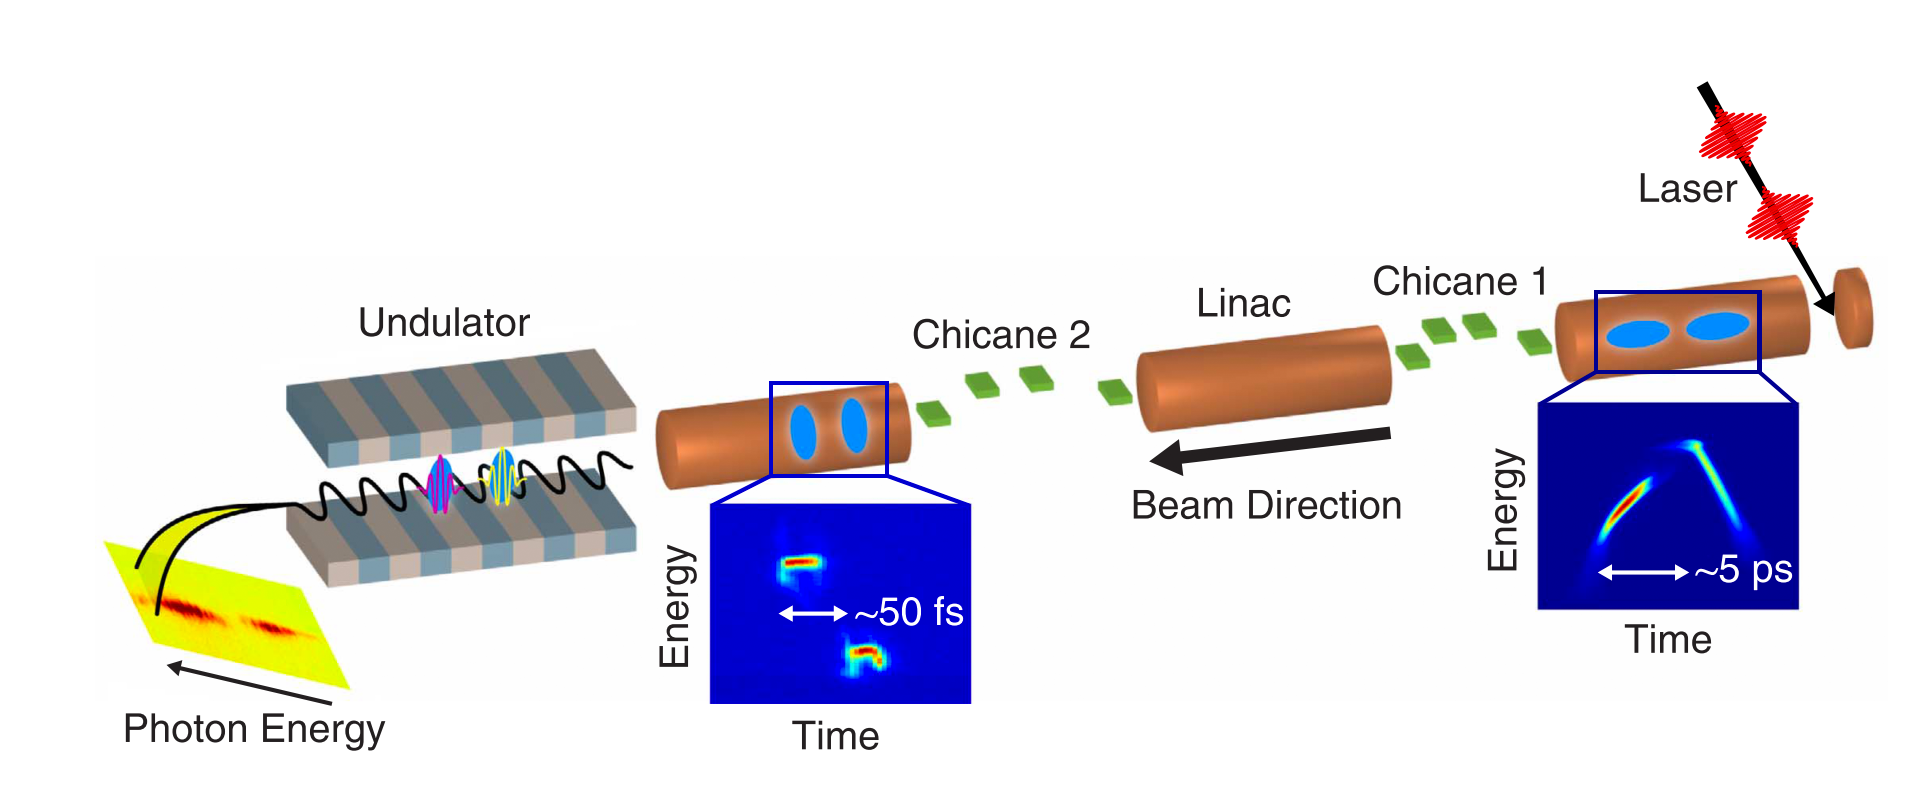
\includegraphics[width=1.00\textwidth]{images/Agos-pump-probe-scheme.png}
	\caption[Schematic setup of a bunch based pump-probe setup.]{Schematic setup of the two bunch, two color pump--probe setup at LCLS. Two laser pulses shot at a cathode create two electron bunches with a delay $\Delta t$ on the picosecond timescale. Two magnetic chicanes compress the bunches such that a delay $\Delta t$ is on the ten femtosecond timescale. Both pulses go through one undulator section and the lasing process is saturated. The relative color separation is on the order of $\SI{1}{\percent}$ between the bunches. From \citep[\href{http://creativecommons.org/licenses/by/4.0/}{\ccby}]{Marinelli-2015-NatComm}.}
	\label{fig:Agos-pump-probe-scheme}
\end{figure}
The second developed accelerator-based X-ray pump-X-ray probe technique at LCLS \citep{Marinelli-2015-NatComm} uses two electron bunches of different energy. A schematic setup of this beam operation can be found in Figure \ref{fig:Agos-pump-probe-scheme}. The electron bunches are created through a double laser pulse that impinges on a photo-cathode. Initially, these two bunches are delayed by a few picoseconds, however, two magnetic chicanes compress the peak current of the electron bunches from \SI{20}{\ampere} to \SI{4}{\kilo\ampere} such that after the acceleration in the linac a time delay on the ten-femtosecond timescale is achieved. Also after the acceleration stage, the electron bunches also have a difference in kinetic energy, i.e., Lorentz factor, $\gamma$. When the electron bunches then travel through the undulator section, both pulses saturate in their lasing process at different colors. For \SI{8.3}{\kilo\electronvolt} photons, both pulses combined can reach pulse energies of \SI{1.2}{\milli\joule}, the color separation is up to \SI{100}{\electronvolt}, and the time separation ranges from $\Delta t_{\text{min}}=\SI{0}{\femto\second}$ to $\Delta t_{\text{max}}=\SI{100}{\femto\second}$. For hard X-rays, this method requires the pump-pulse to have a higher photon energy than the probe-pulse, although their respective intensities may vary. For soft X-rays, the slotted spoiler foil can be used. This enables further control over the electron bunches and allows crossing time zero with both pulses.
%%%
\section{Rare-gas clusters}\label{sec:cluster-theory}
%%%%%%%%
%- Why are rare gas clusters a suitable sample
%%%%%%%%
Clusters have a long history as samples to study the light-matter interaction for a few reasons. In general, their characteristics are well known, they can form interesting states, and their use often has practical purposes \citep{Haberland-1994-Springer}. Generally speaking, clusters are an aggregation of atoms or molecules and vary in size. Their size ranges from a few atoms to mesoscopic sizes such that one can classify a cluster as a bulk material. Rare-gas clusters are a subclass of clusters and they are bound by van der Waals forces, thus they are normally neutral-charged. Single, solid van der Waals clusters typically form in an icosahedral\footnote{An icosahedron is a polyhedron with 20 faces, i.e., a dice with 20 faces.} shape when they are sufficiently small (up to nanometer sized) \citep{Miehle-1989-JCP} and have mostly a fcc-crystal\footnote{fcc is an acronym for face-centered cubic. A very common crystal structure.} structure but exhibit also hcp-crystal\footnote{hcp stands for hexagonal close-packed and is also a crystal structure.} structures \citep{VanDeWaal-1993-JCP,Krainyukova-2006-TSF}. In the present work, superfluid helium clusters (or droplets), solid xenon clusters and a mixture of both have been used as samples as they form a finite system that can be produced and tuned in size easily, they have no energy dissipation in surrounding media and can exist in the gas phase. The creation of homogenous and heterogeneous rare-gas clusters is discussed in the next sub-sections.
%
%
%
\subsection{Production of homogenous clusters: The supersonic gas expansion}\label{sec:homogenous-cluster}
%%%%%%
%- the theory behind rare-gas cluster creation.
%%%%%%
Rare-gas clusters, for example, xenon clusters, can be generated in a variety of ways. In this thesis experiment, rare-gas clusters are created via supersonic expansion by releasing gas from a reservoir through a nozzle into a vacuum. The gas in the reservoir is at a certain stagnation pressure, $p_{0}$, and temperature, $T_{0}$. Typical values for $p_{0}$ are \SI{10}{\bar}, where the mean free path of the atoms is much smaller than the nozzle diameter\footnote{A schematic drawing of the nozzle used in this work can be found in Figure \ref{fig:parker-valve}. See also Equation \eqref{eq:equivalent-nozzle-opening} for non-pinhole nozzle openings.}. This is why many collisions occur in the nozzle during the gas expansion, but collisions do not occur in the free supersonic expansion. The collisions in the nozzle intuitively explain the cluster formation \citep{Lippmann-1984-JCP}, which we will discuss first. We follow the phenomenological discussion with a more detailed description of the supersonic gas expansion and end the section with the empirically derived scaling laws that describe average sizes for rare-gas clusters.\\[1\baselineskip] 
%
In the nozzle, clusters grow through collisions. The collisions can be expressed mathematically through the following reaction formula
\begin{align}
A_{n}+A_{m} \rightleftharpoons A_{n+m}^{*},\quad n,m=1,2,...,\quad \text{collision,}
\intertext{with $n,m$ denoting the number of monomers assembling body $A_{n,m}$. A body $A_{n}$ collides with another body $A_{m}$ and forms a metastable state $A_{n+m}^{*}$ that will dissociate if no subsequent collision deactivates it. This can be formulated as}
A_{n+m}^{*}+M\rightleftharpoons A_{n+m} + M,\quad \text{activation/deactivation},
\label{eq:early-cluster-growth}
\end{align}
where $M$ is a chaperone that can be any kind of third body that adds or removes energy from the system. $M$ can therefore activate or deactivate the system.
%
The initial stages of the cluster growth are driven by monomer addition but as more and more clusters are available, cluster-cluster coagulation starts to dominate the later growth process. This is due to the quantitative increase in small clusters in the generation process that then start to collide. From empirical evidence \citep{Zurek-1980-JCP,Soler-1982-PRL}, we know that clusters solely generated through monomer addition follow a size distribution of an exponential decay with a rather large decay constant, whereas larger clusters that grew through coagulation follow a log-normal distribution. Here, the density of smaller clusters including monomers and dimers decreases as larger clusters are formed of these particles through coagulation.\\[1\baselineskip]
%The mean size of a cluster, i.e., the mean of the log-normal distribution, is given by the parameters of the supersonic gas expansion (see below).
%While we have described a cooling gas in the expansion process it should be noted that the clusters are comparably hot. 
During the entire formation process, binding energy is set free that heats the cluster efficiently. In order to lose energy, the cluster typically evaporates monomers. The evaporation process makes the ultimate temperature of the cluster size-independent, after the clusters have reached a certain minimum size \citep{Farges-1981-SurfSci}.
%Typically, the jet reaches temperatures of a few Kelvin and 
The cluster temperature is heavily dependent on their material, particularly the binding energy. Relevant for this study are the temperature of Xenon cluster\footnote{To put this temperature in perspective, krypton clusters have a temperature of \SI{\sim 50}{\kelvin} and argon clusters \SI{\sim 40}{\kelvin}, when they are created through a supersonic jet expansion, with a certain flight distance, and have a minimum size of 800 atoms \citep{Farges-1981-SurfSci,Gspann-1986-Springer}.}, which is \SI{\sim 75}{\kelvin}, and the fact that xenon clusters are solid as their melting temperature is higher \citep{Gspann-1986-Springer}. For similar reasons, helium-clusters are liquid, which is why they are often called helium droplets. If He-droplets are produced using a cryogenic jet also superfluid helium-droplets can be observed \citep{Gomez-2011-JCP}.\\[1\baselineskip]
%
\begin{figure}
	\centering
		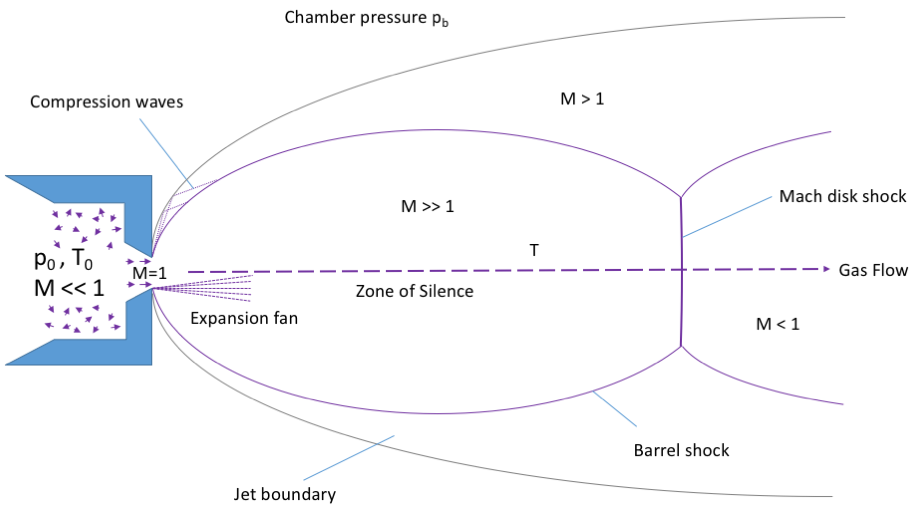
\includegraphics[width=0.80\textwidth]{images/freeJetExpansion.png}
	\caption[Schematic of a supersonic gas expansion into a vacuum.]{Schematic of a supersonic gas expansion into the vacuum. The gas is stored in a reservoir at pressure $p_{0}$, temperature $T_{0}$, and the speed of the gas is thermally distributed $\left(M\ll 1\right)$. As the gas enters the nozzle area, it is accelerated to the speed of sound $\left(M=1\right)$ and as the gas expands, the temperature T drops altering the speed of sound such that the gas now travels supersonically $\left(M\gg 1\right)$. After \citep{Miller-1988-Oxford}.}
	\label{fig:freeJetExpansion}
\end{figure}
%
%Supersonic jet setups typically store gas in a reservoir at a certain stagnation pressure, $p_{0}$, and temperature, $T_{0}$. The gas expands through a nozzle into a vacuum and  Typical values for $p_{0}$ are 10 bars, where the mean free path of the atoms is much smaller than the nozzle diameter\footnote{A schematic drawing of the nozzle can be found in Figure \ref{fig:parker-valve}, $d$. See also Equation \eqref{eq:equivalent-nozzle-opening} for non-pinhole nozzle openings.}. This is why many collisions occur during the expansion in the nozzle and the above described kinetic theory explains the cluster formation. 
To discuss the supersonic expansion in detail, we assume an ideal gas and say that turbulence and the effects of heat conduction are unimportant \citep{Yamada-2001-SciDir,Haberland-1994-Springer}. Figure \ref{fig:freeJetExpansion} shows a schematic drawing of this process. In the reservoir, the velocity distribution of the gas is thermally distributed at a set temperature $T_{0}$. The movement direction of each atom is randomly orientated. For an ideal gas, we can define the enthalpy, $H_{0}$, in the stagnation chamber by
\begin{align}
H_{0}=C_{P}\ T_{0}.
\label{eq:stagnation-enthalpy}
\end{align}
The expansion of the gas through the nozzle is driven by the pressure ratio $p_{b}/p_{0}$. Only when the ratio exceeds a critical value, $G$, the expansion will be supersonic. We note, $G\equiv \left(\left(\gamma + 1\right)/2\right)^{\gamma/\left(\gamma - 1\right)}$, where $\gamma$ is the ratio of specific heats, $\gamma = \tfrac{C_{P}}{C_{V}}$, at constant pressure, $C_{P}$, and volume $C_{V}$. $\gamma$ can be regarded as independent of temperature for atomic gases. In the nozzle, the steady gas flow becomes directed and the enthalpy, $H_{0}$, is converted into kinetic energy, $\tfrac{1}{2}m_{gas} v^{2}$, and a remaining enthalpy, $H$. We can use the conservation of energy and Equation \eqref{eq:stagnation-enthalpy} to write down
\begin{equation}
H_{0}=H+\frac{1}{2}m_{gas} v^{2} = C_{P}\ T+\frac{1}{2}m_{gas}v^{2},
\label{eq:local-temperature}
\end{equation}
with $T$ being the local temperature along the gas flow and $m_{gas}$ the atomic mass of the gas. To simplify, let us define the Mach number, $M\equiv v/c_{s}$, as the ratio of the stream velocity, $v$, and the local speed of sound, $c_{s}$. We can express the local speed of sound as
\begin{equation}
c_{s}=\sqrt{\frac{\gamma\ k_{B}\ T}{m_{gas}}},
\label{eq:local-speed-of-sound}
\end{equation}
where $k_{B}$ is the Boltzmann constant and we can rearrange Equation \eqref{eq:local-temperature} to 
\begin{equation}
T=T_{0}\left(1+\frac{1}{2}\left(\gamma - 1\right)M^{2}\right)^{-1}.
\label{eq:local-temperature-definition}
\end{equation}
Here, the interplay between the Mach number and the local temperature give insight into the directed mass flow versus the remaining thermal energy in the system. As indicated in the Figure \ref{fig:freeJetExpansion}, $M$ increases dramatically along the indicated gas flow direction and that is due to a decrease in $c_{s}$, which is proportional to $\sqrt{T}$ as indicated in Equation \eqref{eq:local-speed-of-sound}. The gas quickly reaches the terminal velocity while the speed of sound is decreasing. We may write the terminal velocity as
\begin{equation}
v_{\infty}=\sqrt{\frac{2 R}{m_{gas}}\left(\frac{\gamma}{\gamma-1}\right) T_{0}},
\label{eq:terminal-velocity}
\end{equation}
with $R$ being the universal gas constant. The expansion speed of the gas gives the name to such types of gas sources, namely supersonic jets. This equation is also useful to calculate gas or cluster flight times, $t_{\text{flight}}=\frac{D}{v_{\infty}}$, if the distance $D$ from nozzle to interaction point is known (see Section \ref{sec:jet-timing}). \\[1\baselineskip]
%
The appearance of the supersonic jet stream (see Figure \ref{fig:freeJetExpansion}) is particularly important for the experimental aspect of delivering the sample to the interaction region. Upon exiting the nozzle, the Mach number increases by a wide margin ($M\gg 1$). This means that the gas travels faster than information in this medium, i.e., the local speed of sound. Here, a \textit{zone of silence} is formed, where the gas flow is not influenced by other particles or boundary conditions.
% As the supersonic flow exits the nozzle, it has to turn around the edge of the nozzle to further expand and it does so by actually creating smaller Mach waves.
At the borders of the zone of silence, $M$ decreases drastically, resulting in dense regions that are called \textit{barrel shock} to the sides and \textit{Mach disk shock} downstream the gas flow \citep{Miller-1988-Oxford}. For an unhindered transport of the gas and clusters to the interaction region, the interaction region needs to be within the zone of silence. We can express the distance from the nozzle to the Mach disk $x_{MD}$ through
\begin{equation}
\frac{x_{MD}}{d}=0.67\sqrt{\frac{p_{0}}{p_{b}}},
\label{eq:distance-of-mach-disk}
\end{equation}
with the nozzle diameter $d$. So, the competing stagnation pressure, $p_{0}$, and the vacuum chamber pressure, $p_{b}$, define the distance of the otherwise static parameters. $p_{b}$ needs to be low enough to drive the Mach disk downstream of the interaction region. By using skimmers and thereby physically separating the jet expansion into separately pumped compartments, the pressure $p_{b}$ can be reduced, hence $x_{MD}$ increased.\\[1\baselineskip]
%
\begin{table}
	\centering
		\begin{tabular}{ | l | l | l | l | l | }
			\hline
			Helium & Neon & Argon & Krypton & Xenon \\ \hline
			3.85 & 185 & 1646 & 2980 & 5554 \\ \hline
		\end{tabular}
	\caption[Parameter $K_{\text{gas}}$ values for rare-gases.]{Parameter $K_{\text{gas}}$ values for rare-gases \citep{Schorb-2012-Thesis}.}
	\label{tab:k-parameter}
\end{table}
The average cluster size\index{cluster size} is very much dependent on the gas type, stagnation temperature $T_{0}$, stagnation pressure $p_{0}$, and the nozzle diameter. An empirically found scaling law\index{scaling law}, named after Hagena\index{Hagena|see {scaling law}} \citep{Hagena-1972-JCP,Hagena-1981-SurfSci,Hagena-1987-ZeitschriftAMC}, can be summarized as follows. The Hagena scaling parameter, $\Gamma^{*}$, reads
\begin{equation}
\Gamma^{*} = K_{\text{gas}} \cdot T_{0}^{0.25x-1.5} \cdot p_{0} \cdot d_{eq}^{x}\quad \left[\si{\micro\meter\milli\bar\per\kelvin}\right],
\label{eq:Hagena-parameter}
\end{equation}
with the gas-specific parameter $K_{\text{gas}}$ that can be found in Table \ref{tab:k-parameter} for some rare-gases, the gas specific parameter $x$ that varies between 0.5 and 1 and is 0.85 for all rare-gases, and the equivalent nozzle opening, $d_{eq}$, that is $d_{eq}=d$ for pinhole sources. For conical nozzles, $d_{eq}$ becomes \citep{Schorb-2012-Thesis}
\begin{equation}
d_{eq} = d\frac{\tan\left(\Phi_{0}\right)}{\tan\left(\Phi\right)} = 0.719 \frac{d}{\tan\left(\Phi\right)},
\label{eq:equivalent-nozzle-opening}
\end{equation}
where $\Phi$ is the half-opening angle of the nozzle and $\Phi_{0}$ is the half-opening of the free gas expansion. $\Gamma^{*}$\index{Hagena!scaling parameter} allows us to estimate the mean cluster size, i.e., the mean amount of accumulated particles per cluster $\left\langle N\right\rangle$, via the following cases
\begin{itemize}
	\item $\Gamma^{*} < 350$, no cluster formation is observed;
	\item $350 < \Gamma^{*} < 1800$, in this region $\left\langle N\right\rangle$ reads \citep{Buck-1996-JChemPhys}
		\begin{equation}
		\left\langle N\right\rangle = 38.4 \left(\frac{\Gamma^{*}}{1000}\right)^{1.64};
		\label{eq:intermediate-hagena-scaling}
		\end{equation}
	\item after $1800 < \Gamma^{*}$, $\left\langle N\right\rangle$ is
		\begin{equation}
		\left\langle N\right\rangle = 33.0 \left(\frac{\Gamma^{*}}{1000}\right)^{2.35}.
		\label{eq:large-hagena-scaling}
		\end{equation}
\end{itemize}
There is a range, where the mean cluster size deviates from Hagena's law \citep{Dorchies-2003-PRA}, and it is the range
\begin{itemize}
	\item $\num{e4} < \Gamma^{*} < \num{e6}$, where $\left\langle N\right\rangle$ becomes
		\begin{equation}
		\left\langle N\right\rangle = 100 \left(\frac{\Gamma^{*}}{1000}\right)^{1.8}.
		\label{eq:dorchies-scaling}
		\end{equation}
\end{itemize}
Note, however, that for larger cluster sizes, the Equation \eqref{eq:large-hagena-scaling} becomes true again \citep{Hagena-1992-RSI,Bush-1998-JPhysChemA}. The average number of atoms, $\left\langle N\right\rangle$, which arrange to a cluster, is in this thesis usually expressed as the radius of a cluster, $r$. In a good approximation, the number of atoms, $\left\langle N\right\rangle$, can be expressed as a cluster radius using the atomic Wigner-Seitz radius, $R_{s}$, as follows. The Wigner-Seitz radius can be noted as \cite{Arbeiter-2010-PRA,Gomez-2011-JCP}
\begin{align}
R_{s} &= \left(\frac{3 M}{4 \pi\, \rho\, N_{A}}\right)^{\frac{1}{3}},
\label{eq:wigner-seitz-radius}
\intertext{where $M$ is the molar mass, $\rho$ is the mass density, and $N_{A}$ is the Avogadro number. $R_{s}$ is typically given in \AA and using the mass density for superfluid He-droplets, $R_{s}^{He}\approx \SI{2.2}{\angstrom}$ and for solid xenon, $R_{s}^{Xe} \approx \SI{1.7}{\angstrom}$. The cluster radius, $r$, can then be noted as,}
\left\langle r\right\rangle &= R_{s} \left\langle N\right\rangle^{\frac{1}{3}},
\end{align}
assuming the cluster agglomerates symmetrically in three dimensions.\\[1\baselineskip]
%
Experiments using supersonic jets for cluster generation are sometimes performed with pulsed valves to decrease cost and gas load in the overall system. Upon opening and closing of the valve, the gas density can vary. This affects the cluster size and one would expect to see smaller clusters. It has been observed that one finds smaller clusters in the beginning of the pulse but in the \textit{afterpulse}\index{afterpulse}, one finds giant clusters that exceed the above-described scaling laws due to the effects when closing the valve \citep{Rupp-2014-JCP}.\\[1\baselineskip]
%
Supersonic jets generally create clusters of different sizes. This size distribution is centered around $\left\langle N\right\rangle$ and for solid rare-gas clusters this distribution is a log-normal distribution. The size distribution can be an experimental challenge, especially when size-dependent effects are investigated. Historically, electron diffraction \citep{Farges-1981-SurfSci,Bartell-1986-ChemRev} has been used to determine the mean cluster size, mean temperature, and mean geometry. Today, free electron lasers allow the determination of the size of a single cluster through a diffraction image \citep{Rupp-2012-NJP}, and by measuring enough single clusters, one can reproduce size distributions of a supersonic jet as shown in Figure \ref{fig:size-distributions}.
%
%
%
%
%
%
\subsection{Creation of heterogeneous clusters: The pickup principle}\label{sec:heterogeneous-cluster}
%%%%%%%%%%%%%%%%%
%- Heterogeneous clusters, e.g. He Xe\\
%- Do you have literature on that?
%%%%%%%%%%%%%%%%%
\begin{figure}
	\centering
		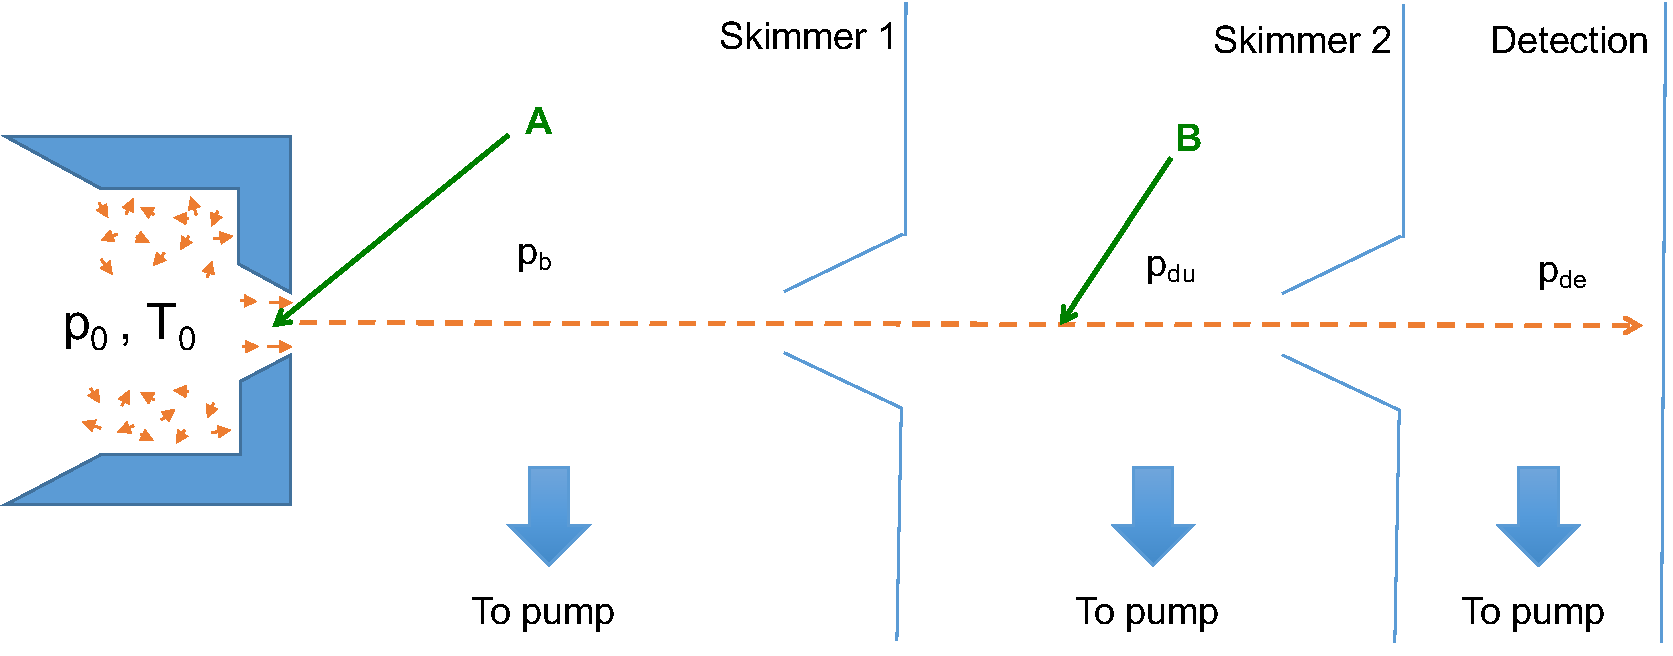
\includegraphics[width=0.80\textwidth]{images/pick-up.pdf}
	\caption[Schematic of a pickup (gas-)source.]{Schematic setup to generate heterogeneous clusters through pickup. Thereby is a cluster generated via supersonic gas expansion, which is doped at regions marked A or B. In region A, the dopant gas is mixed in the nozzle such that it becomes part of the nucleus. In region B, the cluster condenses atoms on its surface from the background gas of the chamber with pressure $p_{\text{du}}$. The cluster can be detected upon evaporation, e.g., due to contact with the chamber, through the pressure $p_{\text{de}}$. After \citep{Gough-1985-JChemPhys,Haberland-1994-Springer}.}
	\label{fig:pickupPrinciple}
\end{figure}
A possibility to create heterogeneous clusters is through the principle of picking-up atoms or molecules \citep{Haberland-1994-Springer}. Figure \ref{fig:pickupPrinciple} illustrates pickup regions that are typically used in an experiment. Mainly, there are two different places where the cluster encounters a dopant material; one, monomers are added to the cluster in region A of Figure \ref{fig:pickupPrinciple}, which represents the nozzle of a supersonic source and can be achieved by, e.g., co-expanding a gas-mixture; two, they can be picked up by a cluster in region B, for example, through an increased chamber pressure $p_{du}$ with the dopant material. If clusters encounter atoms or molecules in the nozzle region A, they can become part of the cluster formation and can be found inside of solid clusters \citep{Gough-1985-JChemPhys}. If atoms or molecules are picked up in region B, they typically stick to the surface of solid clusters. If a liquid or superfluid cluster picks up a dopant, it may move within the droplet \cite{Hartmann-1995-PRL}. Since the traversing cluster in region B is much larger and heavier than a colliding monomer, the trajectory is not affected significantly. Ar-clusters with $\left\langle N\right\rangle = \num{5.9e9}$ particles can pick-up \SI{0.05}{\percent} as many SF$_{6}$ molecules with chamber pressures of $p_{du}=\SI{2e-3}{\pascal}$ over a pickup length of a few centimeters \citep{Gough-1985-JChemPhys}. At these low pressures, picking up atoms or molecules in region B requires less gas load on the system but is also less efficient than picking up in region A. To increase the pickup levels in region B, a gas cell with two openings for the cluster beam can be used. The cell contains the gas well and allows higher doping pressures, without putting too much gas-load on the overall system \cite{Gomez-2014-Science}. In this work, gaseous xenon was picked up by superfluid helium droplets in region B using a gas cell.\\[1\baselineskip]
%
To understand the doping process further, the following considerations are useful. When a cluster and a dopant\index{dopant} bond, the binding energy that is specific to the materials is added to the system. This is similar to the cluster growth process itself. The cluster will lose this energy through evaporation of monomers \citep{Gomez-2011-JCP}. The loss of particles through evaporative cooling is dependent on the ratio of binding energies of the two materials and can be expressed as 
\begin{equation}
N_{\text{Evaporated from cluster}} \approx \frac{\epsilon_{\text{cluster}}}{\epsilon_{\text{dopant}}},
\label{eq:evaporated-amount}
\end{equation}
with the binding energy of the cluster $\epsilon_{\text{cluster}}$ and of the dopant $\epsilon_{\text{dopant}}$. In this thesis, where a helium droplet is doped with xenon atoms, we may use the binding energies of helium, $\epsilon_{He}\approx \SI{0.6}{\milli\electronvolt}$, and of xenon, $\epsilon_{Xe}\approx$ \SI{0.15}{\electronvolt} \citep{Gomez-2011-JCP,Gomez-2014-Science}, to estimate that approximately 250 helium atoms evaporate by picking up 1 xenon atom.\\[1\baselineskip]
%
Now we can extend this idea to estimate the number of picked-up atoms, if we were to know the number of atoms in the cluster before and after the pickup area. An estimate of the initial mean cluster-size, i.e., $\left\langle N_{\text{cluster}}\right\rangle$, can be reached through the scaling laws\footnote{As already established the actual cluster size produced with a supersonic jet will vary, hence the average cluster size $\left\langle N_{\text{cluster}}\right\rangle$.} as discussed in Section \ref{sec:homogenous-cluster}. An estimate of the cluster size after the pickup can be established through measuring the partial pressure of the cluster material without the pickup, $p_{\text{de}}$, for example, in the detection chamber when the particle jet hits a wall and evaporates\footnote{For example with a residual gas analyzer.} (see Figure \ref{fig:pickupPrinciple}), and the partial pressure with pickup, $\Delta p_{\text{de}}$. The relative difference $\tfrac{\Delta p_{\text{de}}}{p_{\text{de}}}$ then scales with \cite{Gomez-2014-Science}
\begin{equation}
\left\langle N_{\text{dopant}}\right\rangle \approx \frac{\epsilon_{\text{cluster}}}{\epsilon_{\text{dopant}}} \cdot \frac{\Delta p_{\text{de}} \left\langle N_{\text{cluster}}\right\rangle}{p_{\text{de}}},
\label{eq:average-dopant}
\end{equation}
such that the mean amount of picked up atoms, $\left\langle N_{\text{dopant}}\right\rangle$, can be estimated.
%%%
%\section{Introduction into X-ray scattering}\label{sec:scattering-theory}
%%%%%%%%%%%%%%%%%%%%%
%- Starting with Maxwell equations (this would be coming from the far end, I might be able to go into Guiniers formalism earlier. Depending on space.)\\
%- Mathematical model for electromagnetic wave\\
%- Kramers-Kronig relations\\
%- Mie scattering in a nutshell
%%%%%%%%%%%%%%%%%%%%%%%
%
\section{Fundamental processes of soft X-rays and nanoparticles}\label{sec:light-matter-interaction}
\begin{figure}
	\centering
		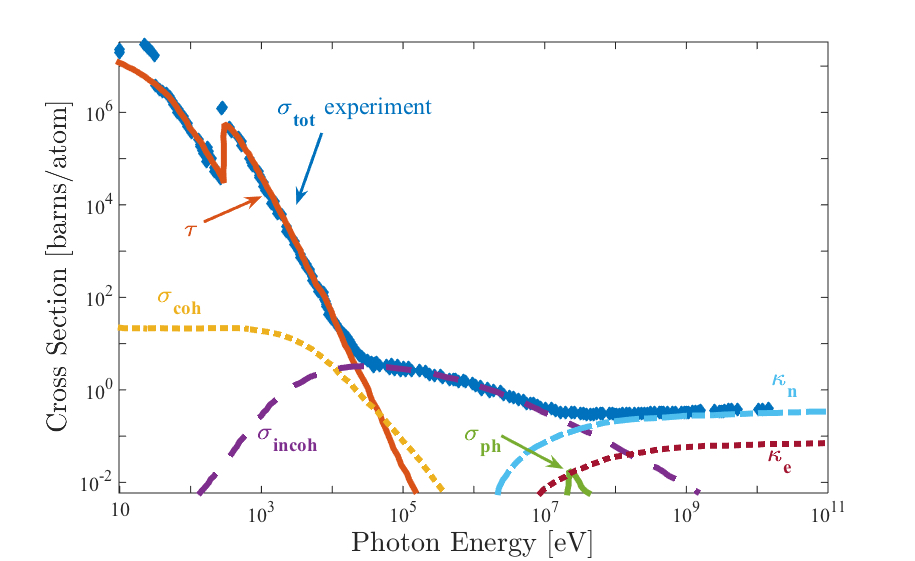
\includegraphics[width=0.80\textwidth]{images/absorption-cross-section-carbon-ken.jpg}
	\caption[Total cross-section of atomic carbon.]{The total cross-section of atomic carbon, $\sigma_{\text{tot}}$, as a function of energy. Several processes add to, $\sigma_{\text{tot}}$: $\tau$, is the photoionization; $\sigma_{\text{coh}}$, is coherent scattering; $\sigma_{\text{incoh}}$, is the incoherent scattering; $\sigma_{ph}$, is photonuclear absorption; $\kappa_{n}$, and $\kappa_{e}$, are pair-production events. At the experimental photon energy of \SI{837}{\electronvolt}, the dominant effects are photoionization and coherent scattering. From \citep{Ferguson-2016-PhD,Williams-2009-xb}.}
	\label{fig:absorption-cross-section-carbon-ken}
\end{figure}
%
%We may break down the light-matter interaction into five categories, 1) coherent-elastic scattering (see sub-Section \ref{sec:saxs}), 2) resonant processes (absorption, see sub-Section \ref{sec:absorption}), 3) incoherent scattering (Compton effect), high-energy physics effects of 4) pair production, and 5) absorption effects with the nucleus. The effects are dependent on the wavelength and the cross-sections for  effects 3-5 are so small that they can be neglected in the soft X-ray regime. We will therefore concentrate the following sub-sections on points 1-2 and restrict ourselves to the for the experiment necessary theory.
Nanoparticles respond to intense X-ray radiation by scattering or absorbing the rays \cite{Als-Nielson-2011-JWS}. Figure \ref{fig:absorption-cross-section-carbon-ken} shows the most probable processes in the X-ray wavelength range. For soft X-rays, the processes are dominated by the photoionization process and the coherent and elastic scattering. Therefore, Section \ref{sec:absorption} discusses photoionization and the resulting core-hole decay processes; Section \ref{sec:saxs} discusses the coherent elastic scattering of an electron and extends this concept to the scattering and imaging of a nanoparticle; and Section \ref{sec:generalized-index-of-refraction} generalizes the refractive index. The chapter follows the discussion in Reference \citep{Als-Nielson-2011-JWS} and avoids effects that have negligible cross-sections, such as the Compton effect, the pair-production, and the scattering from the nucleus.
%This section will give  a brief introduction into the elastic scattering of X-rays with matter. The actual scattering process is very complex as it is an interplay of coherent, incoherent and elastic, inelastic processes. Fortunately, we can reduce the scattering description to its main process: The coherent and elastic scattering. In other words, we neglect Compton scattering (incoherent), any kind of absorption processes (inelastic) and effects form the scattering of multiple particles. We will then start this section by looking at the small angle scattering of atoms and continue on to extended objects such as clusters. The section is rounded off by an introduction to the inverse problem and basic algorithm ideas to overcome the issue of phase retrieval.
%Photons can also be absorbed by atoms in which case an electron get either excited to another state or ionized. At X-ray wavelengths matter typically gets ionized in the inner shells. Upon absorption a cascade of relaxation processes begins and the now ionized atom finds the new most energetic favorable state. These processes are particularly dependent on the wavelength of the incident photons but also the type of atom. This chapter is devoted to these processes and particular the absorption process is described in Section \ref{sec:absorption} and the relaxation processes in \ref{sec:relaxation}.
%
%
%
\subsection{Photoionization and core-hole decay}\label{sec:absorption}
%
\begin{figure}
	\centering
		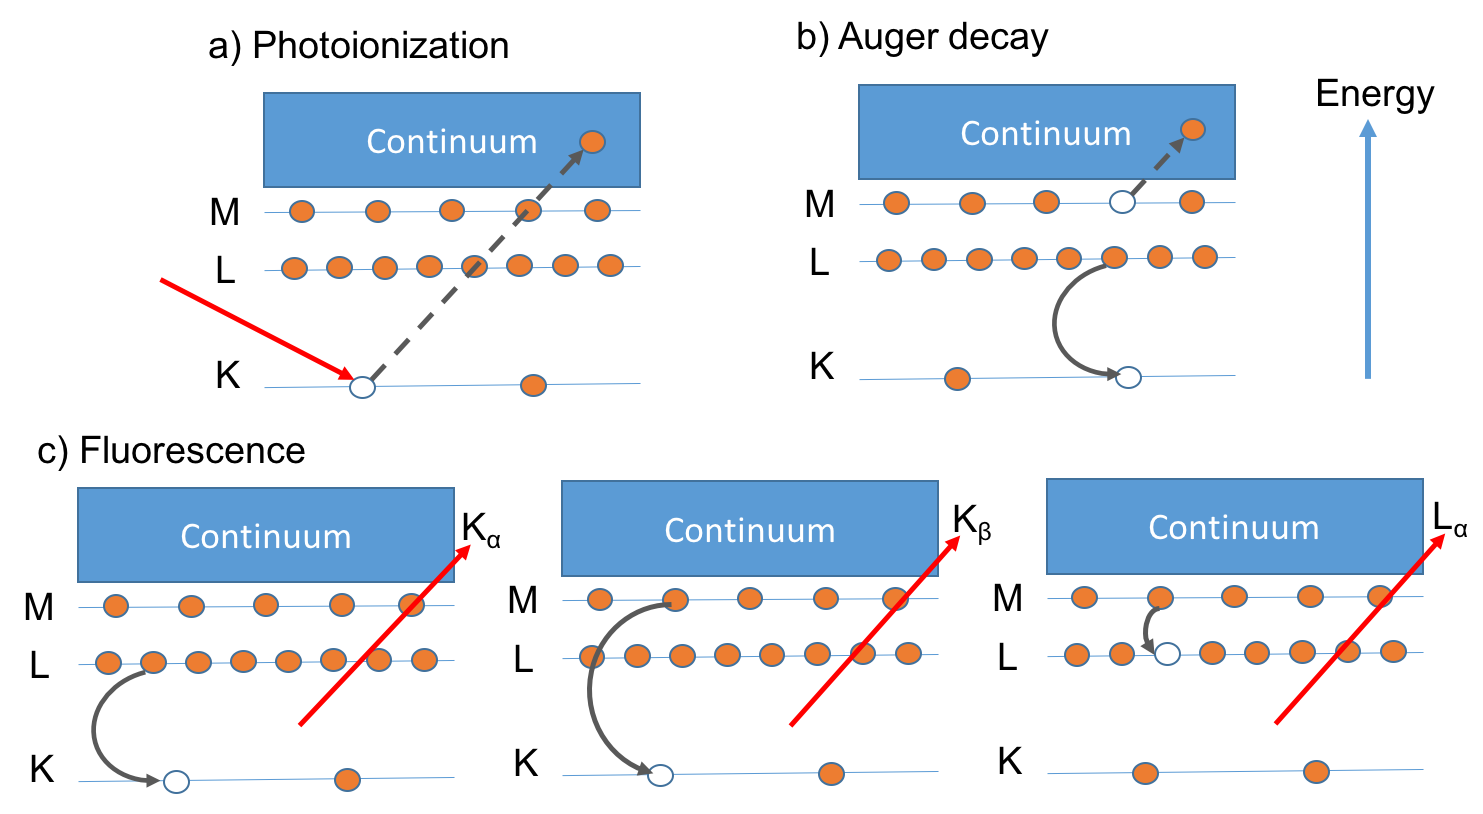
\includegraphics[width=0.80\textwidth]{images/el-relaxation.png}
	\caption[Schematic illustration of fundamental light-matter processes.]{Schematic of fundamental light-matter processes. a) Photoionization: Describes a direct emission of a K-shell electron after absorbing an X-ray photon. b) Auger decay: A core-hole decay, where a K-shell hole is filled with an electron from the L-shell and the remaining energy is released through emission of an electron in an outer shell. c) Fluorescence: An electron hole is filled with an electron from an outer shell and the remaining energy is released through photons. After \citep{Als-Nielson-2011-JWS}.}
	\label{fig:el-relaxation}
\end{figure}
%
Given the photon energies of soft X-rays, atoms are typically core-ionized when absorbing a soft X-ray photon, which is depicted in Figure \ref{fig:el-relaxation}a) Photoionization. This typically leaves the atom in an excited state. In order to emit energy, the \textit{electron core-hole} usually decays according to the schematics in Figure \ref{fig:el-relaxation}b) Auger decay and c) Fluorescence, whereby the Auger decay is the dominant process for the parameters discussed in this thesis. These processes are discussed in more detail below.\\[1\baselineskip]
%
%
%
\begin{figure}
	\centering
		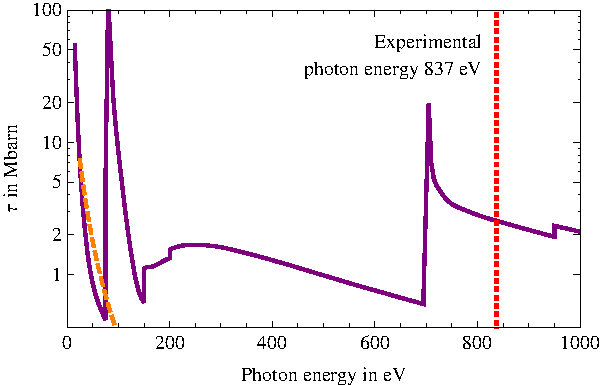
\includegraphics[width=0.80\textwidth]{images/photoionization.pdf}
	\caption[Total absorption cross-sections for helium and xenon.]{Total absorption cross-sections $\tau$ in megabarn for xenon (purple line) and helium (orange, dashed line). The photon energy of the described experiment is \SI{837}{\electronvolt} (red, dashed line). Data points from \citep{Elettra-2016-Website,Yeh-1985-AtmDat,Yeh-1993-GBSP}.}
	\label{fig:photoionization}
\end{figure}
%
%Figure \ref{fig:photoionization} shows the total absorption cross-sections $\tau$ for xenon and helium for various photon energies. The photon energy of the experiment was $\SI{837}{\electronvolt}$. For helium, the photon energy is much greater than the binding energy and thus the absorption cross-section is low. For the tightly bound electrons in xenon, the absorption cross-section is relevant as the photon energy is near the atomic levels. The absorption cross-section shows a resonant-type behavior, when the photon energy would be directly on an atomic level. To get a better understanding of the absorption cross-section with regard to atomic levels, Table \ref{tab:xenon-photoionization-cross-section} and \ref{tab:helium-xenon-ionization} show the differential photo-absorption cross sections and ionization potentials for various energy levels and ionization configurations at the experimental photon energy $\SI{837}{\electronvolt}$ for xenon and helium. The calculations were performed with the Los Alamos Atomic Physics code based on \citep{Cowan-1981-Cal}.\\[1\baselineskip]
Photoionization is the process where an atom or molecule is transformed into an ion through absorption of a photon and emission of an electron (see Figure \ref{fig:el-relaxation}a). Here, the photon energy must be higher than the ionization threshold. Figure \ref{fig:photoionization} shows the total absorption cross-sections, $\tau$, for xenon and helium for various photon energies. $\tau$ is strongly dependent on the photon energies as resonant behavior occurs near absorption edges.
%
\begin{table}
	\centering
		\begin{tabular}{ | c | c | c | c | }
			\hline
			Shell & Subshell & Cross-section & subshell ionization \\
				&	& in Mb & potential in eV \\ \hline
			K & 1s & - & 34630.0 \\ \hline
			L & 2s & - & 5466.4  \\ 
			\ & 2p & - & 4899.1 \\ \hline
			M & 3s & - & 1153.3  \\ 
			\ & 3p & - & 965.4 \\ 
			\ & 3d & 2.2505 & 682.7 \\ \hline
			N & 4s & 0.0305 & 223.7 \\ 
			\ & 4p & 0.1247 & 161.8 \\ 
			\ & 4d & 0.2587 & 68.2  \\ \hline
			O & 5s & 0.0040 & 27.3  \\ 
			\ & 5p & 0.0120 & 12.5  \\ \hline
		\end{tabular}
	\caption[Subshell absorption cross-sections and ionization potentials for xenon.]{Subshell absorption cross-sections and ionization potentials for certain electronic configurations of xenon at \SI{837}{\electronvolt}. Calculations performed with \citep{los-alamos-2016,Cowan-1981-Cal}.}
	\label{tab:xenon-photoionization-cross-section}
\end{table}
%It appears that certain energy levels, or here subshells if one disregards the hyperfine structure\footnote{A shift in energy levels due to interaction of electrons with the nucleus \citep[see][p~166~ff.]{Demtroder-2005-Springer}.}, tend to have a higher absorption cross-section than others. This brings us back to the picture of the forced harmonic oscillator, where an electron is driven by a light field. If the frequency of the light field is close to the eigenfrequency of the bound electron, in other words, if the energy of a photon is close to the energy level of a bound electron, the system is in resonance and absorption is highly likely. As the photon energy and electron level energy differ, the system is off resonance and it is less likely to absorb a photon. As energy levels in atoms are discrete, electrons can only be excited from one energy level to another or need a certain (minimal) ionization energy\index{ionization!energy} to ionize an atom and excite an electron into the continuum. Therefore, the likelihood of a core-electron that is strongly bound being ionized is by far the most probable using X-rays.
It is therefore useful to state the absorption cross-sections per atomic subshell\footnote{Disregarding the hyperfine structure, which is a shift in atomic energy levels due to interaction of electrons with the nucleus \citep{Demtroder-2005-Springer}.}. Table \ref{tab:xenon-photoionization-cross-section} shows the subshell absorption cross-sections and ionization potentials for xenon. If the photon energy is below the ionization threshold of a subshell, this subshell cross-section becomes negligibly small. In this thesis experiment's photon energy of \SI{837}{\electronvolt}, xenon dominantly absorbs photons in the 3d-subshell.
\begin{table}
	\centering
		\begin{tabular}{ | c | c | c | c | }
		\hline
%			Configuration & ionized subshell & Cross-section (Mbarn) & Helium ionization potential in eV \\ \hline
			El. Configuration, & Ionization & Cross-section  & subshell ionization  \\
			and ionized subshell & of subshell & $\tau$ in Mbarn & potential in eV \\ \hline
			He\textsuperscript{+0},\ 1s2 & 1s2 & 0.0007 & 24.4 \\ \hline
			He\textsuperscript{+1},\ 1s1 & 1s1 & 0.0005 & 54.4 \\ \hline
			Xe\textsuperscript{+0},\ 5p6 & 3d10 & 2.2505 & 682.7 \\ \hline
			Xe\textsuperscript{+1},\ 3d9 & 3d9 & 2.1487 & 733.6 \\ \hline
			Xe\textsuperscript{+1},\ 5p5 & 3d10 & 2.2443 & 693.7 \\ \hline
			Xe\textsuperscript{+2},\ 5p4 & 3d10 & 2.2390 & 705.9 \\ \hline
		\end{tabular}
	\caption[Absorption cross-sections and ionization potentials for xenon and helium]{Total absorption cross-sections $\tau$ and ionization potentials for certain electronic configurations. Calculations performed with \citep{los-alamos-2016,Cowan-1981-Cal}.}
	\label{tab:helium-xenon-ionization}
\end{table}
%To discuss the parameters that are most applicable to this thesis, a comparison of the most probable transition at the photon energy \SI{837}{\electronvolt} is given for helium and xenon in Table \ref{tab:helium-xenon-ionization}. The ionization energies change drastically, whether a core electron or a less tightly bound electron is ionized. As per absorption cross-sections, helium can be considered transparent and xenon atoms have a much larger absorption cross-section. 
After ionization, the electronic structure of an atom changes, which alters ionization energies and absorption cross-sections. Table \ref{tab:helium-xenon-ionization} shows total absorption cross-sections for helium and xenon in various electronic configurations. The number of ionization configurations is numerous and the table gives the reader merely an impression of the change for some early ionization steps of helium and xenon in this thesis experiment. The cross-section and ionization potential calculations are performed with the Los Alamos Atomic Physics Codes \cite{los-alamos-2016} that are based on Reference \citep{Cowan-1981-Cal}.\\[1\baselineskip]
%
%
%
\begin{figure}
	\centering
		a)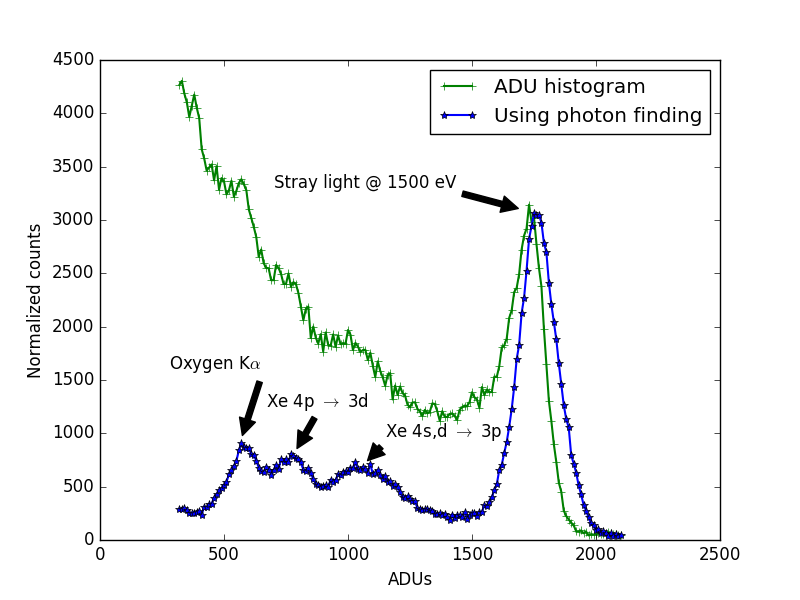
\includegraphics[width=.47\textwidth]{images/pnCCD-histogram.png}
		b)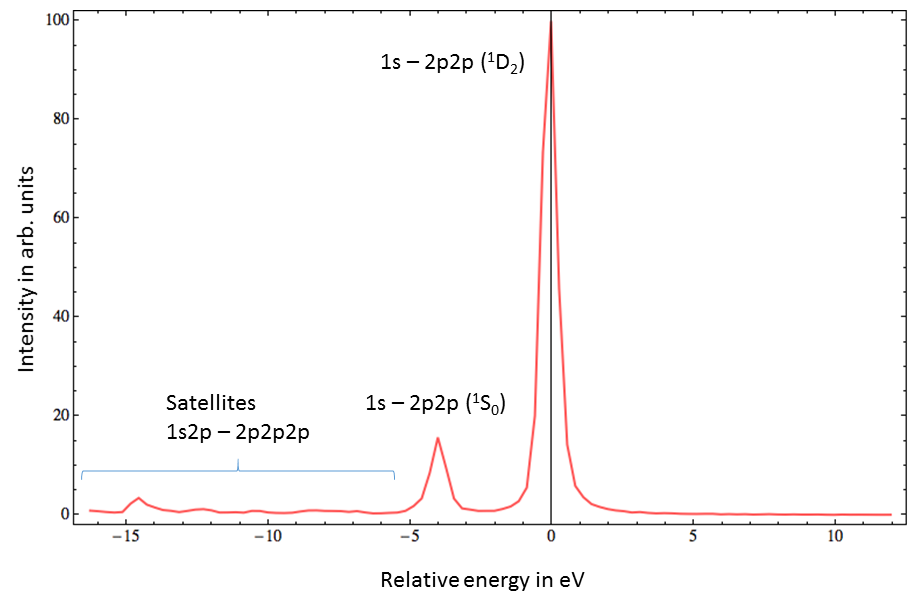
\includegraphics[width=.47\textwidth]{images/auger-spectra.png}
	\caption[Fluorescence peaks from xenon and neon K-LL Auger spectrum.]{a) Fluorescence spectra of xenon and oxygen, which are excited by \SI{1.5}{\kilo\electronvolt} photons from the LCLS. The spectra are recorded with pnCCD detectors \citep{Bucher-2016-Unpublished} and the green curve is an ADU histogram of the raw pnCCD image. The blue curve uses a coalescent photon finder \cite{Foucar-2016-JAC} and the peaks are identified as in \cite{Rudek-2012-NatPho}. b) Partial K-LL Auger spectrum with rel. energy 0 corresponding to \SI{804.5}{\electronvolt}. Spectrum is measured with a hemispherical analyzer \citep{Bucher-2014-Unpublished} and the peaks are identified as in \citep{Krause-1970-PhysLettA}.}
	\label{fig:pnCCD-histogram}
\end{figure}
%
Far off resonance, the Auger decay is a two-step process (see Figure \ref{fig:el-relaxation}b) \cite{schmidt-1997}: one, an outer shell electron is emitted into the continuum, the so-called \textit{Auger-electron}\footnote{Named after the French physicist Pierre Auger.}; two, another electron in the atom simultaneously fills the electron-hole. \textit{Auger decay} typically occurs on a few femtoseconds timescale after core-ionization \citep{Buth-2003-JCP}. Emitted Auger-electrons have discrete energies depending on the combination of electrons involved in the process. One can use this attribute to, for example, identify elements or calibrate energies. The right panel of Figure \ref{fig:pnCCD-histogram} shows a partial K-LL\footnote{This nomenclature means a single core-hole in the K-shell decays into two holes in the L-shell.} Auger spectrum from neon illuminated by \SI{1050}{\electronvolt} photons from the LCLS and measured with a hemispherical analyzer \citep{Bucher-2014-Unpublished}. In this example, neon is ionized in the K-shell and an electron-hole in the 1s shell is created. An electron from the L-shell fills the 1s hole and another electron from the L-shell, the Auger electron, is emitted into the continuum. As there are a variety of electronic configurations that can be involved in this process, multiple peaks appear for similar occupation configurations, e.g., 1s - 2p2p. More complex structures, called satellites, appear when the atom is already ionized, for example, when an atom has a hole in the L-shell and photoionization creates another hole in the K-shell, this leads to KL-LLL satellites \cite{schmidt-1997}. Doubly K-ionized atoms will produce so-called hypersatellites \cite{Briand-1971-PRL}, which occur in the intense soft X-ray pulses of LCLS \cite{Young-2010-Nature,Berrah-2011-PNAS}. The transition can also be of the same shell and is then called a Coster-Kronig transition, for example, the N-NN Coster-Kronig transitions in xenon \cite{Coster-1935-Physica}.\\[1\baselineskip]
%
Fluorescence is the emission of light by a material that has been photoexcited (see Figure \ref{fig:el-relaxation}c). If the material is has been core-ionized, the fluorescence decay can result in the emission of X-rays with distinct energies, for example, the for many materials well-known K$_\alpha$-, K$_\beta$-, and L$_\alpha$-lines. These can be used for, e.g., element identification, or chemical analysis. The left panel of Figure \ref{fig:pnCCD-histogram} shows fluorescence peaks that contribute to the background signal when diffraction images are taken with the pnCCD detectors (see Section \ref{sec:pnCCD}). In our case, fluorescence often occurs on the pico- to nanosecond timescale \citep{Berezin-2011-ChemRev} and it is therefore typical that the Auger decay rates beat the fluorescence decay rates \cite{Young-2010-Nature}. However, the rates vary depending on the material and its electronic configuration such that in intense XFEL pulses these rates are expected to change as the electrons are stripped of the atom \cite{Ho-2014-PRL}.
%
%In this measurement, xenon atoms and residual oxygen atoms have been illuminated with 1500 eV photons from the Linac Coherent Light Source and the fluorescence photons have been measured with the LAMP pnCCD detectors that are described in Section \ref{sec:pnCCD}. 
%The green curve is a ADU histogram of the pixel-detector using the detector calibrations described in Section \ref{sec:pnccd-corr}. The blue curve additionally uses a coalescent-photon finding algorithm\index{algorithm!coalescent-photon finding} looks for pixels above a certain threshold and includes neighboring pixels above a certain, lower threshold, thus correcting the measured signal to yield a proper ADU count per photon.\\[1\baselineskip]
%
%
%
%Similarly to the estimate made in Equation \eqref{eq:absorption-cross-section}, it is very unlikely for an atom to absorb more than two photons in one pulse of a free electron laser, which is why we only consider the most probably transitions here to get an understanding how the absorption cross-sections change.\\
% \begin{table}
% 	\centering
% 		\begin{tabular}{ | c | c | c | c | }
% 		\hline
% 			El. Configuration, & Ionization & Cross-section  & subshell ionization  \\
% 			and ionized subshell & of subshell & $\tau$ in Mbarn & potential in eV \\ \hline
% 			Xe\textsuperscript{+0},\ 5p6 & 3d10 & 2.2505 & 682.7 \\ \hline
% 			Xe\textsuperscript{+1},\ 3d9 & 3d9 & 2.1487 & 733.6 \\ \hline
% 			Xe\textsuperscript{+1},\ 5p5 & 3d10 & 2.2443 & 693.7 \\ \hline
% 			Xe\textsuperscript{+2},\ 5p4 & 3d10 & 2.2390 & 705.9 \\ \hline
% 		\end{tabular}
% 	\caption{caption. Calculations based on \citep{Cowan-1981-Cal}.}
% 	\label{tab:xenon-ionization}
% \end{table}{}
%In the experiment described in the following chapters, the photon energy is explicitly chosen to have a comparably high absorption cross-section for xenon -- but is off the absorption resonance --, a comparably low absorption cross-section for helium, and a wavelength short enough to receive high resolution images through coherent diffraction imaging. In such a setting, xenon is most likely to absorb X-rays and helium can be considered transparent.
%
%
%
%
%
\subsection{From Thomson scattering to diffractive imaging}\label{sec:saxs}
%%%%%%%%%%
%- Switch to Guiniers approximation and description\\
%- Work towards small angle scattering of small particles\\
%- Particular spheres\\
%- Discuss extreme positions
%%%%%%%%%%%
The elastic scattering of photons off the nanoparticle is discussed in detail below. Let us therefore first consider the elastic scattering of a free electron, or \textit{Thomson scattering}, as a result of being accelerated in an electro-magnetic field. Then, we use these insights and proceed to the scattering of an atom followed by the scattering of an extended object with a continuous electron density. We end the section with some considerations that are relevant for this work.\\[1\baselineskip]
%We can describe an electric field of a light wave semi-classically via the following expression \citep{Als-Nielson-2011-JWS}
%\begin{equation}
%\vec{E}(\vec{r},t) = \vec{\epsilon} E_{0} e^{i \left(\vec{k}\cdot\vec{r}-\omega_{0}t\right)},
%\end{equation}
%with $\vec{r}$ the Cartesian coordinate vector, $\hbar \vec{k}$ the momentum of a photon, $\hbar \omega_{0}$ the energy of a photon, $E_{0}$ the incident amplitude, and \vec{\epsilon} an unit vector due to the polarization. $\vec{\epsilon}$ obeys $\vec{\epsilon}\cdot\vec{k}=\vec{k}\cdot\vec{E}=\vec{k}\cdot\vec{B}=0$, with the magnetic field $\vec{B}$, as the electro-magnetic waves are transverse. To avoid delving into a quantum mechanic description, we shall call \vec{k} the wavevector.
Let us introduce the electric field of an incident wave $E_{in}=E_{0}e^{-i\omega t}$ that irradiates an electron. The electron is accelerated in this electric field and emits radiation similarly to a small dipole antenna. We can write this radiated electric field as \citep{Als-Nielson-2011-JWS}
\begin{equation}
E_{rad}(R,t)=-\underbrace{\left(\frac{e^2}{4\pi \epsilon_0 m c^2}\right)}_{r_{0}}\ E_{in}\ \frac{e^{i k R}}{R} \cos\left(\psi\right),
\label{eq:radiated-by-electron}
\end{equation}
with $k$ being the usual wave-number, $R$ being the distance from the source of radiation, $\psi$ being the observation angle, and $r_0$ being the \textit{Thomson scattering length}, or the \textit{classical electron radius}. $r_0$ can be written in practical units as
\begin{equation}
r_0 = \frac{e^2}{4\pi \epsilon_0 m c^2} = 2.82\cdot 10^{-5}\si{\angstrom},
\label{eq:thomson-scattering-length}
\end{equation}
where $-e$ is the charge of an radiating electron, $m$ is the mass of the electron, $c$ is the speed of light, and $\epsilon_0$ is the permittivity of free space.\\[1\baselineskip]
%
Now we would like to understand the cross-section of this scattering process better. We can establish a differential cross-section, $\left(\tfrac{d\sigma}{d\Omega}\right)$, which follows the same concept of the already discussed example in Equation \eqref{eq:absorption-cross-section}. The only difference is that we now consider a scattered intensity, $I_{sc}$, of an incident flux, $\left(I_{0}/A_{0}\right)$, into a solid angle, $\Delta \Omega$. We may express this as
\begin{align}
\left(\frac{d\sigma}{d\Omega}\right)&=\frac{I_{sc}}{\left(I_{0}/A_{0}\right)\Delta\Omega}=\frac{\lvert E_{rad}\rvert^2 R^2}{\lvert E_{in}\rvert^2}=r_0^2 \cos^{2}\left(\psi\right),
\label{eq:scattering-crosssection}
\end{align}
which is also called the differential cross-section for Thomson scattering. By integrating over the full angular space, the total cross-section for Thomson scattering, $\sigma_{T}$, results in
\begin{align}
\sigma_{T} = \left(\frac{8\pi}{3}\right) r_{0}^{2} = \SI{0.665}{\barn}.
\label{eq:Thomson-cross-section}
\end{align}
%\begin{align}
%\left(\frac{d\sigma}{d\Omega}\right)&=\frac{\left(\text{Number of X-rays scattered per second into $\Delta \Omega$}\right)}{\left(\text{Incident flux}\right)\left(\Delta\Omega\right)}=\frac{I_{sc}}{\left(I_{0}/A_{0}\right)\Delta\Omega},
%\label{eq:scattering-crosssection}
%\end{align}
%with $A_{0}$ being the covered area of the incident beam. If an electro-magnetic wave encounters an electron, we can describe the scattering semi-classical by imagining how an electron starts to oscillate once it sees an incoming electric wave. The electron then functions as a dipole antenna eventually radiating the wave into a certain solid angle $\Delta \Omega$. Depending on the polarization of the incident beam we can reduce Equation \eqref{eq:scattering-crosssection} to \citep{Als-Nielson-2011-JWS}
%\begin{align}
%\left(\frac{d\sigma}{d\Omega}\right)&=r_{0}^{2}P,
%\intertext{with the classical electron radius $r_{0}=2.82\ 10^{-5}\text{\AA}$ and the polarization factor P}
%P&=\begin{cases}
%1& \text{vertical scattering plane},\\
%\cos^{2}\left(\Psi\right)&\text{horizontal scattering plane}, and\\
%\frac{1}{2}\left(1+\cos^{2}\left(\Psi\right)\right)& \text{unpolarized source.}
%\end{cases}
%\end{align}
We can now move on and use this knowledge for atoms, where we have Z electrons. To describe electrons in an atom, let us introduce an electron density $\rho_{e}\left(\vec{r}\right)$ that describes the probability density of electrons in an atom. Figure \ref{fig:X-ray-scattering} illustrates the scattering process by one atom. An incident beam, with wave-vector $\vec{k}$, is elastically scattered at the origin, O, into a wave with $\vec{k}'$ such that $\lvert \vec{k}\rvert=\lvert \vec{k}'\rvert$. 
%We can describe this phase difference, $\Delta \Phi\left(\vec{R}\right)$, of the waves scattered at $\vec{R}$ and the origin by
It is useful to define the \textit{wave-vector transfer}\index{wave-vector!transfer}, $\vec{Q} = \vec{k}-\vec{k}'$, which we can write in terms of the \textit{scattering angle}, $\Theta$, as
\begin{equation}
\lvert \vec{Q}\rvert=2 \lvert \vec{k}\rvert \sin\left(\frac{\Theta}{2}\right)=\frac{4 \pi}{\lambda}\sin\left(\frac{\Theta}{2}\right),
\label{eq:Q-scattering-angle}
\end{equation}
where $\lambda$ is the wavelength of the scattering light.\\[1\baselineskip]
\begin{figure}
	\centering
		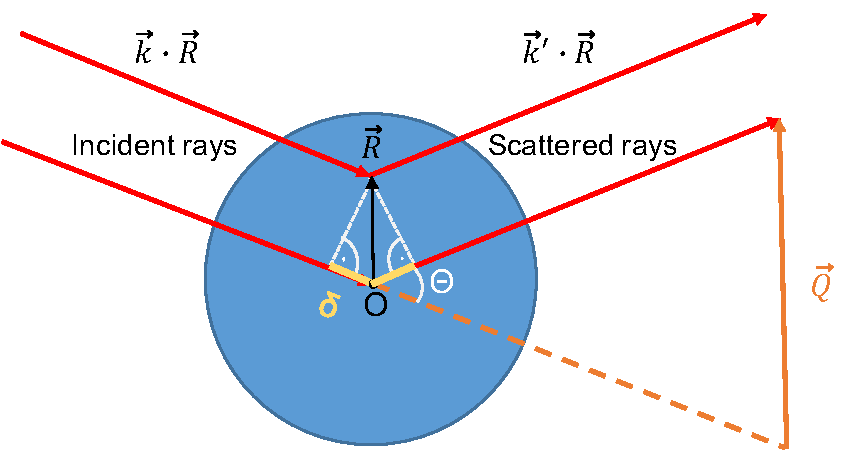
\includegraphics[width=0.80\textwidth]{images/X-ray-scattering.pdf}
	\caption[Principle of scattering rays of an atom.]{Principle of scattering rays of an atom. After \citep{Als-Nielson-2011-JWS,Guinier-1955-JWS}.}
	\label{fig:X-ray-scattering}
\end{figure}
%
A volume element $d\vec{R}$ of the atom at $\vec{R}$ will now scatter waves proportional to its electron density, which we can express by $-r_{0}\ \rho\left(\vec{R}\right)d\vec{R}$. At scattering angle $\Theta=\vec{Q}=0$, the \textit{atomic scattering factor}, $f^{0}$, can be shown to be
\begin{equation}
f^{0}\left(\vec{Q}\rightarrow 0\right)=Z,
\label{eq:transform-number-of-particles}
\end{equation}
because all scatterers are in phase. As we increase the scattering angle $\Theta$, a wave that is scattered at the origin, O, and one at $\vec{R}$ have an optical path difference of $2 \delta$. This difference in path length results in a phase difference, $\Delta \Phi$, in the wavefront. $\Delta \Phi$ can be expressed as 
\begin{equation}
\Delta \Phi = \left(\vec{k}-\vec{k}'\right)\cdot \vec{R} = \vec{Q}\cdot \vec{R}.
\label{eq:phase-difference}
\end{equation}
We may multiply a \textit{phase factor}, $e^{i \vec{Q}\cdot \vec{R}}$, to the contribution of the scattered field, $-r_{0}\ \rho\left(\vec{R}\right)d\vec{R}$, to argue that the volume elements start to scatter out of phase. As a consequence and in the limit of $\vec{Q}\rightarrow\infty$, the atomic form factor is thus $f^{0}\left(\vec{Q}\rightarrow\infty\right)=0$. Let us gather these phenomenological arguments, integrate over them to obtain the total scattering volume, and note
\begin{equation}
-r_{0} f^{0}\left(\vec{Q}\right)=-r_{0}\int\rho_{e}\left(\vec{R}\right)e^{i \vec{Q}\cdot \vec{R}}d\vec{R}.
\label{eq:scattering-integral}
\end{equation}
This important result is called the atomic form factor and is here written in units of $-r_{0}$. It can be understood as a Fourier transformation of the electron density of an atom.\\[1\baselineskip]
%
Let us continue with the scattering of a molecule or cluster that consists of multiple atoms. We can label the atoms in such an object by
\begin{equation}
F^{0}\left(\vec{Q}\right)=\sum_{\vec{R}_j}f_{j}^{0}\left(\vec{Q}\right)e^{i \vec{Q}\cdot \vec{R_{j}}},
\label{eq:scattering-factor-object}
\end{equation}
with the atomic form factors $f_{j}^{0}\left(\vec{Q}\right)$ for the $j$'th atom and call $F^{0}$ the single particle \textit{structure factor}. Similar to above, an electron density can be found for the molecule or cluster by labeling the atoms \citep{Vartanyants-2001-JOP} and for coherent and monochromatic radiation, the scattered amplitude, $A(\vec{Q})$, of a nanoparticle can be written in the kinematical approximation\footnote{Sometimes called the weak-scattering limit, where multiple scattering effects are neglected.} as 
%Strictly speaking and as defined in \eqref{eq:scattering-factor-object}, $F^{object}\left(\vec{Q}\right)$ and $f_{j}^{Q}\left(\vec{Q}\right)$ is $\vec{Q}$ dependent. As this is inconvenient, let us consider the following evidence in order to neglect this dependency. In the angular range of $\vec{Q}$, where $F^{Object}\left(\vec{Q}\right)$ is not 0, $f_{j}^{Q}$ can be considered constant \citep[see][p. 6-7]{Guinier-1955-JWS}. In human hemoglobin, the range in which the molecule scattering length $F^{Object}\left(\vec{Q}\right)$ is not 0, the carbon atomic form factors change less than $0.4$\%. Neglecting this $\vec{Q}$ dependency in $f_{j}^{Q}$ allows us to describe the scattering length of extended objects $F^{Object}\left(\vec{Q}\right)$ via one continuous electron density $\rho_{e}\left(\vec{r}\right)$, where certain volume elements $d\vec{r}$ scatter proportional to their electron density $\rho_{e}\left(\vec{r}\right)$. Let us write down the more convinient expression for the scattering length of an object
\begin{equation}
A(\vec{Q})=\int \rho\left(\vec{R}\right) e^{i \vec{Q}\cdot R}d\vec{R},
\label{eq:scattered-amplitude}
\end{equation}
where $\rho\left(\vec{R}\right)$ is the electron density of the scattering nanoparticle. This operation can again be interpreted as a Fourier transformation of the single particle’s electron density. But, only scattered intensities can be measured with, e.g., a CCD detector. So, the scattered intensity in a diffraction pattern can be expressed by
\begin{equation}
I_{sc}\left(\vec{Q}\right)=I_{0}\lvert A(\vec{Q})\rvert^{2},
\label{eq:scattered-intensity}
\end{equation}
where $I_{0}$ is the intensity of an incident beam\footnote{Here, we make use of the Born approximation and the intensity of the incident beam becomes constant, which holds true in the kinematical approximation}. Unfortunately, the operations on the amplitude, $\lvert A(\vec{Q})\rvert^{2}$, eliminate the phase factor, such that merely an inverse Fourier transformation cannot be used to reconstruct the real-space electron density from measured intensities. This is known as the \textit{inverse problem} and can be solved by iterative phase-retrieval algorithms that we will discuss in Section \ref{sec:phase-retrieval}.\\[1\baselineskip]
%
Let us now make use of above's theory and address the scattering of a rare-gas cluster, as they will reoccur throughout this thesis. We may thus express an electron density of the desired object and Fourier transform it into reciprocal space to understand diffraction patterns better. Due to current resolution limitations\footnote{Considering experimental details from Chapter \ref{ch:exp_setup}}, we may approximate the shape of a few nanometer-sized cluster with a sphere. The density, $\rho$, of a hard sphere with radius, $r$, can be expressed by 
\begin{align}
\rho\left(\vec{R}\right)&=\begin{cases}
\rho& \text{for $r \geq \lvert\vec{R}\rvert \geq 0$},\\
0&\text{for $r > \lvert\vec{R}\rvert$}.
\end{cases}
\label{eq:el-density}
\end{align}
Using this equation, we can solve the integral in Equation \eqref{eq:scattered-amplitude} by making use of spherical coordinates,
\begin{align}
A_{\text{Sphere}}\left(\vec{Q}\right) &= \rho \int_{0}^{\pi}\int_{0}^{2\pi}\int_{0}^{r} R^{2}  \sin\left(\Theta\right) e^{i \lvert\vec{Q}\rvert R \cos\left(\Theta\right)} dR d\Theta d\Phi,\\
&=\frac{4 \pi \rho}{\lvert\vec{Q}\rvert^{3}}\left(\sin\left(\lvert\vec{Q}\rvert r\right)-\lvert\vec{Q}\rvert r\cos\left(\lvert\vec{Q}\rvert r\right)\right).
\label{eq:scattering from sphere}
\end{align}
This result can be exploited to determine the size of a spherical particle, i.e., a cluster, using local minima in the diffraction pattern\footnote{Equation \eqref{eq:scattering from sphere} can be solved numerically for the distance between the first two minima, $\vec{Q}_{\text{min}^{n}}$ and $\vec{Q}_{\text{min}^{n+1}}$, such that $r=\frac{3.24}{\vec{Q}_{\text{min}^{n+1}}-\vec{Q}_{\text{min}^{n}}}$.} or through a numerical fit of the resulting curve. The envelope function of this curve is the from small-angle scattering well-known Porod's law \cite{Sinha-1988-PRB}. For the here discussed spheres, the envelope function is proportional to
\begin{equation}
I(\lvert\vec{Q}\rvert \gg 0)\propto \lvert\vec{Q}\rvert^{-4},
\label{eq:porods-law}
\end{equation}
and for this thesis very useful in estimating the expected scattering.\\[1\baselineskip]
%
\begin{table}
	\centering
		\begin{tabular}{ | c | r | }
		\hline
			El. Configuration, & Scattering cross-section \\
			and ionized subshell & $\sigma_{\text{coh}}$ in barn \\ \hline
			He\textsuperscript{+0},\ 1s2 & 2.55  \\ \hline
			He\textsuperscript{+1},\ 1s1 & 0.65  \\ \hline
			Xe\textsuperscript{+0},\ 5p6 & 1874.36  \\ \hline
			Xe\textsuperscript{+1},\ 3d9 & 1813.56  \\ \hline
			Xe\textsuperscript{+1},\ 5p5 & 1814.68  \\ \hline
			Xe\textsuperscript{+2},\ 5p4 & 1754.08  \\ \hline
		\end{tabular}
	\caption[Atomic scattering factors for helium and xenon.]{Atomic scattering cross-sections for certain electronic configurations at \SI{837}{\electronvolt} photon energy. From \citep{Ho-2016-PC}.}
	\label{tab:helium-xenon-el-scattering-crossection}
\end{table}
%
The total atomic scattering cross-sections, $\sigma_{\text{coh}}$, for helium and xenon in some electron configurations can be found in Table \ref{tab:helium-xenon-el-scattering-crossection}. The scattering cross-section calculations are based on Equation \eqref{eq:scattering-integral} and are $\sigma_{\text{coh}}=r_{0}^{2}\lvert f^{0}\rvert^{2}$ \citep{Ho-2016-PC}. Xenon atoms scatter dominantly over helium atoms as xenon's scattering cross-section is over \num{700} times larger than helium's. This means for the diffraction images of mixed HeXe-clusters that xenon atoms contribute as much as helium atoms to the scattering when the doping level is \SI{\sim 0.14}{\percent}. Also upon ionization, xenon atoms scatter dominantly. Singly ionized xenon atoms have their scattering cross-section reduced by only \SI{\sim 3}{\percent} and singly ionized helium atoms have their scattering cross-section reduced by \SI{\sim 75}{\percent} compared to the scattering cross-section of their neutral electron configurations. For the same ionization level in xenon, e.g., $Xe\textsuperscript{+1}$, but different electron configurations, the scattering cross-section varies only on the order of \SI{\sim 0.05}{\percent}, which is a small effect compared to the change in the scattering cross-section when xenon becomes increasingly ionized.
%It is interesting to see that although a xenon atom has only 27 times more electrons than a helium atom the scattering factor $f^{0}$ of neutral xenon is over 900 times stronger than helium. Upon ionization, the absolute changes in $f^{0}$ of helium are therefore smaller compared to xenon. The relative change in helium of $f^{0}$ after one electron is ionized is \SI{\sim 30}{\percent}, thus (ionized) helium barely scatters. As xenon has multiple occupied subshells, the scattering factors of different ionized subshells are shown in Table \ref{tab:helium-xenon-el-scattering-crossection}. As discussed, it is most likely to ionize the xenon 3d subshell, however, within a few femtoseconds subsequent relaxation processes\footnote{See the following Section \ref{sec:relaxation}.} lead to different ionization configurations, for example a double ionized 5p subshell. For the scattering factor, there is little change whether the 3d or 5p subshell becomes ionized and the change in $f^{0}$ is only 
%s xenon has 54 electrons, the relative change upon ionization of one electron in $f^{0}$ is only \SI{3}{\percent}. Xenon is therefore a much stronger scatterer than helium and xenon still scatters well upon ionization of inner or outer shell electrons.  
%
%
%
\subsection{Generalized index of refraction}\label{sec:generalized-index-of-refraction}
The last section established that an electron was accelerated by a light field and radiated as a result.
%in th
%by disregarding a variety of effects through Fourier transforming the electron density of an atom.
%As we have already discussed, the electron is accelerated by the lightfield
%As we established, we can compare the photon-electron interaction to the analogue of the forced harmonic oscillator, where an electric field drives a (bound) electron.
But, it is not only the light field that drives the electron, also the electron has an effect on the light field. Ultimately, this effect changes how rays scatter off extended objects and therefore our interpretation of recovered real-space electron densities. The atomic form factor can be corrected for these effects with the so-called \textit{dispersion corrections}. Single particle imaging software suites, such as Condor \cite{Hantke-2016-JCR}, can make full use of these corrections, which is why the following considerations may be helpful. However, we do not derive this topic to its full extent as it can be found in \citep[][p. 55 ff]{Attwood-2007-CUP}, but we qualitatively compare the equation for the complex refractive index, $n\left(\omega\right)$, to the resonant description of the atomic form factor, $f\left(\vec{Q},\omega\right)$. For simplicity, we reduce the following considerations to the case of forward scattering, where $\lvert\vec{Q}\rvert=\Theta=0$.\\[1\baselineskip]
%
As a wave propagates through a medium, for example, from air through water, it changes direction according to \textit{Snell's law} \citep{Als-Nielson-2011-JWS}. Here, a medium is attributed a refractive index,\index{refractive index}
\begin{equation}
n=\frac{c}{v_{\text{phase}}},
\label{eq:refractive-index}
\end{equation}
where $v_{\text{phase}}$ is the phase velocity that changes inside the material. $n$ is wavelength dependent and for visible wavelengths, it ranges between 1.2 and 2, which indicates $v_{\text{phase}}<c$. X-rays usually have a refractive index of $n<1$. As a result, one usually speaks of a \textit{phase advance} when an X-ray field traverses an object, for example, a \SI{20}{\nano\meter} thick silicon nitride membrane causes an estimated phase advance of \SI{20}{\degree} in \SI{32}{\nano\meter} light \cite{Chapman-2006-NatPhys}.
%The phase velocity of light, $v_{\text{phase}}$, is slower than the speed of light in vacuum $c$ due to interacting with electrons. We can describe this effect via the refractive index $n\equiv c/v_{phase}$.
Another aspect, when a light wave is traveling through, e.g, from air through water, is the attenuation of the amplitude. When a light wave travels through a medium along the $Z$-axis, its amplitude is reduced by $e^{\mu Z/2}$, with $\mu$ being the \textit{absorption coefficient}, for example, the transmission of the \SI{20}{\nano\meter} silicon nitride membrane is \SI{44}{\percent} at the wavelength of \SI{32}{\nano\meter} \cite{Chapman-2006-NatPhys}.
%Particularly, when the energy of the photons is higher than the binding energies of electrons there must be absorption.
%Imagine an electro-magnetic wave propagating in a medium with the above considerations. The wave travels along the $Z$-axis and can be written as \citep{Als-Nielson-2011-JWS,Attwood-2007-CUP}
The amplitude of an electro-magnetic wave that propagates through a medium along the $Z$-axis with wave number $k$ and the above considerations can be expressed as \citep{Attwood-2007-CUP}
\begin{equation}
e^{i n k Z}= \underbrace{e^{i k Z}}_{\text{vacuum propagation}} \underbrace{e^{i \left(\delta\right)k Z}}_{\text{phase shift}} \underbrace{e^{-\beta k Z}}_{\text{decay}},
\label{eq:wave-in-medium}
\end{equation}
where $n$ is the complex refractive index, $\delta$ is its real part resulting in a phase shift of the wave, and $i \beta=i \mu/(2 k)$ is the imaginary part resulting in a decline of the amplitude of the wave. The complex refractive index, $n$, is thus usually written as
\begin{equation}
n=1-\delta+i\beta.
\label{eq:complex-refractive-index}
\end{equation}
But, the refractive index can also be written in terms of the atomic form factor. For this, let us imagine electrons in an atom. The electron's response to being driven by a light field is reduced depending on their binding energies. This can be denoted as $f^{'}$. The bound electrons can also be photoionized, which can be accounted for by an imaginary factor, $i f^{''}$, similar to above. These two resonant effects are called dispersion corrections to the non-resonant atomic scattering factor, $f^{0}$. Let us include these corrections to the atomic scattering factor\index{dispersion correction!complex} and note
%These above considerations also apply to the atomic form factor and we may write the atomic form factor including the dispersion corrections 
\begin{equation}
f\left(\vec{Q},\omega\right)=f^{0}\left(\vec{Q}\right)+f'\left(\omega\right)+i f''\left(\omega\right).
\label{eq:scattering-factor-dispersion-corr}
\end{equation}
Above resonance $\omega$, bound electrons can be largely seen as free electrons such that $f'\left(\omega\right)\rightarrow 0$ and $f''\left(\omega\right)\rightarrow 0$. Close to resonance, $f'\left(\omega\right)$ and $f''\left(\omega\right)$ can become large factors.\\[1\baselineskip]
%
We can compare Equation \eqref{eq:complex-refractive-index} to Equation \eqref{eq:scattering-factor-dispersion-corr} and note the complex refractive index through the atomic form factor as \citep{Als-Nielson-2011-JWS}
\begin{equation}
n= 1- \frac{2\pi \rho_{atom}r_{0}}{k^{2}}\left(f^{0}\left(\vec{Q}=0\right)+f'\left(\omega\right)+i f''\left(\omega\right)\right),
\label{eq:eq:complex-refractive-index-atomic-factors}
\end{equation}
with the atomic number density, $\rho_{atom}$. The real and imaginary parts of the refractive index then read
\begin{align}
\delta &= \frac{2 \pi \rho_{atom} r_{0}}{k^{2}}\left(f^{0}\left(\vec{Q}=0\right)+f'\left(\omega\right)\right),\quad \text{and}\\
\beta &= - \left(\frac{2\pi \rho_{atom}r_{0}}{k^{2}}\right)f''\left(\omega\right),
\label{eq:delta-and-beta}
\end{align}
with
\begin{equation}
f''\left(\omega\right)=-\left(\frac{k}{4\pi r_{0}}\right)\tau,
\label{eq:f-2-definition}
\end{equation}
where $\tau$ is the absorption cross-setion.
%
%
%
%\subsection{Charge migration}\label{sec:relaxation}
%\\So far we have looked at X-ray induced processes from atoms. Extended objects, whether a bio-molecule or a cluster, will respond differently than just the atoms they consist of. Nanometer-sized objects will develop a distinct character due to their electronic bond with other particles. This includes rare-gas clusters that are weakly bound Van der Waals forces. We shall explore this behavior in the next Section \ref{sec:ionizatin-of-ext-obj}.
%
%
%
%
\section{Clusters in intense soft X-ray pulses}\label{sec:ionizatin-of-ext-obj}
%%%%%%%%%%%%%%%%%%%
%- Short introduction coming from inelastic scattering
%%%%%%%%%%%%%%%%%%%
The response of a cluster upon irradiation with light often differs from just the atomic response. In the soft X-ray region, the ionization of clusters is initially founded by the ionization of atoms, but the sample environment plays a dominant role in the overall response \cite{Schorb-2012-PRL,Ferguson-2016-SciAdv}. As discussed in Section \ref{sec:cluster-theory}, clusters have testbed environment properties that allow studying effects ranging from atomic, to molecular, and to bulk material attributes. This is why they are an ideal sample to control light-driven many-particle processes \citep{Fennel-2010-RMP}. In Section \ref{sec:nanoplasma-expansion}, we summarize how rare-gas clusters respond to femtosecond long, high-intense X-ray pulses and reflect on recent experiments; Section \ref{sec:tampered-layers} discusses how tamper layers slow the nanoplasma expansion.
%
%
%
\subsection{Formation and expansion of a nanoplasma}\label{sec:nanoplasma-expansion}
%%%%%%%%%%%%%%%%%%%%%%%%
%- Step by step explanation on the formation of a nanoplasma
%%%%%%%%%%%%%%%%%%%%%%%%
\begin{figure}
	\centering
		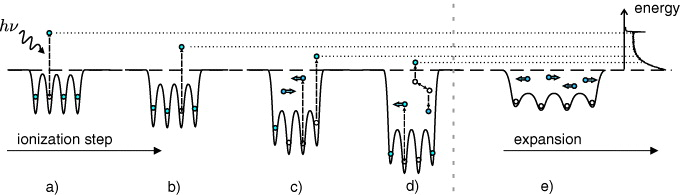
\includegraphics[width=1.00\textwidth]{images/nano-plasma-schematic.jpg}
	\caption[Schematic of the nanoplasma formation and expansion.]{Schematic of the nanoplasma formation and expansion. Step a) X-ray photons ionize the atoms of a cluster. b) Subsequent \textit{multistep ionizations}\index{ionization!multistep} try to relax the electronically excited system, deepening the Coulomb potential of the cluster. Step c) shows a deepened Coulomb potential of the cluster, due to which the multistep ionization becomes (partially) frustrated and electrons are trapped in the potential. In step d) trapped electrons collide and start to thermalize. Collisions can lead to emission of trapped electrons. d) The superheated nanoplasma starts to expand. From \citep[\href{https://creativecommons.org/licenses/by/3.0/}{\ccby}]{Arbeiter-2011-NJP}.}
	\label{fig:nano-plasma-schematic}
\end{figure}
%Let us recapture the scattering and absorption effects discussed in last section Section \ref{sec:light-matter-interaction}. Equation \eqref{eq:scattered-amplitude} indicates how the diffracted amplitude of a nanoparticle can be calculated. Although we disregard inelastic or incoherent processes, the modulo of the amplitude is close to actual measured scattering patterns. However, if we consider the resonant effects discussed in Section \ref{sec:absorption}, it should be clear that the structure factor of a nanoparticle is affected by the dispersion corrections $f'\left(\omega\right)$ and $f''\left(\omega\right)$ that reduce the atomic scattering length, $-r_{0}f^{0}\left(\vec{Q}\right)$. On the one hand, a dominating change in the atomic scattering length is driven by the absorption process that we introduced via the imaginary dispersion correction $i f''\left(\omega\right)$. Upon ionization, the atomic scattering factors, $f^{0}\left(\vec{Q}\right)$, change as the absorption cross-sections start to vary. These small changes are indicated in Table \ref{tab:helium-xenon-ionization} and such processes are exptected to occur on the few femtoseconds timescale, on which the ionization dynamics occur. Additionally, due to photoionized electronsin the atom, the atomic scattering factors change on the few femtoseconds timescale. Such small changes are indicated in Table \ref{tab:helium-xenon-el-scattering-crossection}. On the other hand, there are X-ray induced effects that change the scattering behavior of the collective of atoms, i.e., the cluster. We know from previous experiments \citep{Gorkhover-2016-NatPho} that these changes are related to the nanoplasma expansion and can significantly affect diffraction patterns.\\[1\baselineskip]
%
%Let us follow Figure \ref{fig:nano-plasma-schematic} and \citep{Arbeiter-2011-NJP,Bostedt-2010-JPB} in the next five steps to get an understanding of the nanoplasma formation.
%The nanoplasma formation and subsequent expansion summarize the processes that are responsible for sample damage in diffractive imaging due to highly intense X-ray pulses \cite{Ditmire-1996-PRA}. 
When nanoparticles are irradiated with intense soft X-rays, they form a plasma \cite{Ditmire-1996-PRA}. Due to the finite size of these systems, they are called nanoplasmas. Nanoplasma formation therefore describes the radiation damage processes in typical diffractive imaging experiments. The importance of imaging biological nanoparticles thus lead to much research in the past \cite{Ditmire-1996-PRA,Fennel-2010-RMP,Bostedt-2016-RMP,Bostedt-2012-PRL,Bostedt-2010-JPB,Mikaberidze-2008-PRA,Peltz-2014-PRL} that is still ongoing. This section first discusses nanoplasma formation and expansion of clusters in intense soft X-rays. The discussion then summarized recent experiments that study the nanoplasma evolution and some remarks for this thesis are made.\\[1\baselineskip]
%This section first discusses the nanoplasma formation and expansion of clusters in soft X-rays, then discusses the \textit{electronic damage} and \textit{structural damage} that are imposed in nanoparticles, summarizes recent experiments that study the nanoplasma evolution, and ends with some remarks for this thesis.\\[1\baselineskip]
%
For soft X-rays, nanoplasma formation\index{nanoplasma!formation} and expansion of clusters is schematically shown in Figure \ref{fig:nano-plasma-schematic} and the following steps describe it in more detail \citep{Arbeiter-2011-NJP,Bostedt-2010-JPB}. Step a) the cluster is strongly ionized. Step b), further ionization through emission of photo electrons and Auger electrons lead to a \textit{multistep ionization}\index{ionization!multistep} that deepens the Coulomb potential\index{Coulomb potential} \citep{Wabnitz-2002-Nature,Laarmann-2004-PRL,Bostedt-2008-PRL}. Step c), the multistep ionization is suppressed or, so-called, \textit{frustrated} because the Coulomb potential depth is larger than the excess energies of photo- and Auger electrons. The emitted electrons are now trapped in the cluster potential and are \textit{quasi-free}. As a result, the cluster forms a nanoplasma\footnote{Plasma is another state of matter, similar to solid, liquid and gaseous, where molecular bonds dissociate and positive and negative particles are present in increasing numbers.}. Step d), the kinetic energies of the trapped electrons is initially defined by the discrete excess energies of, e.g., the Auger electrons, but collisions with other particles lead to a kinetic energy distribution that is similar to thermal distributions and can be measured via the spectra of emitted electrons \citep{Laarmann-2005-PRL,Bostedt-2010-NJP}. Step e) An \textit{hydrodynamic expansion} and \textit{Coulomb explosion} are the key mechanisms that now drive an expansion of the cluster until the cluster ultimately disintegrates.\\[1\baselineskip]
%
Both expansion mechanisms reasonably describe the expansion process, are not mutually exclusive, and mostly depend on sample size and irradiation technique. Regarding the sample size, large clusters tend to efficiently trap electrons in their deep Coulomb potentials that thermalize efficiently, which leads to an expansion that is rather driven by hydrodynamic forces due to comparably high electron temperatures. It has been shown that electrons thermalize on the attosecond timescale and that the energy transfer to the ions can be as fast as 50 fs \citep{Arbeiter-2010-PRA}. Small clusters trap photo- and Auger-electrons less efficiently and electrons are free such that the heating process is suppressed. In this case, the ions see the repelling force due to Coulomb interaction of like charges \citep{Lezius-1998-PRL}.\\[1\baselineskip]
%
The nanoplasma formation is dependent on the wavelength that excites the cluster. We focus here on the soft X-ray wavelength range but to give an idea of wavelength dependent aspects in the nanoplasma formation the following can be said. For optical to ultraviolet (UV) pulses, strong field ionization can lead to ionization of clusters and a subsequent nanoplasma expansion \citep{Springate-2000-PRA}. In the vacuum-ultraviolet (VUV) range, \textit{inverse Bremstrahlung heating} leads to efficient energy absorption in clusters and the ionization is driven by collisions inside the strongly coupled plasma \citep{Wabnitz-2002-Nature}. In the extreme-ultraviolet (XUV) to soft X-ray range, direct photoionization and subsequent multistep ionization become the main driver of the ionization, as described above.\\[1\baselineskip]
%It remains to discuss the radiation intensity, which affects the ultimately achieved charge-state combination. The more intense the radiation is, the more energy is absorbed by the cluster. For the nanoplasma this determines the electron temperature and possibly the expansion speed.
%Following a similar line of argumentation, low energy ionizing photons allow efficient trapping of photo and Auger electrons, thus favorable conditions for a hydrodynamic expansion. Conversely, high photon energies\footnote{Meaning hard X-ray with wavelenghs on the {\AA}ngstrom length scale as soft X-rays have similar photon energies as trapping potentials and multistep ionization deepens the Coulomb potential enough.} lead to more atomic excess energy such that more electrons overcome the trapping potential, thus favorable conditions for a Coulomb expansion. However, this line is very element dependent and atoms with large atomic mass, such as Xenon\footnote{Find ionization energies for specific subshells in Table \ref{tab:xenon-photoionization-cross-section} and deepened Coulomb potential ionization energies after ionization of Xe, here Xe$^+1$ and Xe$^{+2}$ for different subshell ionization configurations, in Table \ref{tab:helium-xenon-ionization}.} would require photon energies $E_{ph}$ of $5.5keV\ll E_{ph} < 34.6k eV$ or $34.6keV\gg E_{ph}$ and since mostly the immediate process upon photon absorption is wavelength dependent and the electron trapping of the majority of subsequent multistep ionizations will be mostly dependent on the cluster size.\\
%
%
%
%\subsection{Imaging of transient states}
\begin{figure}
	\centering
		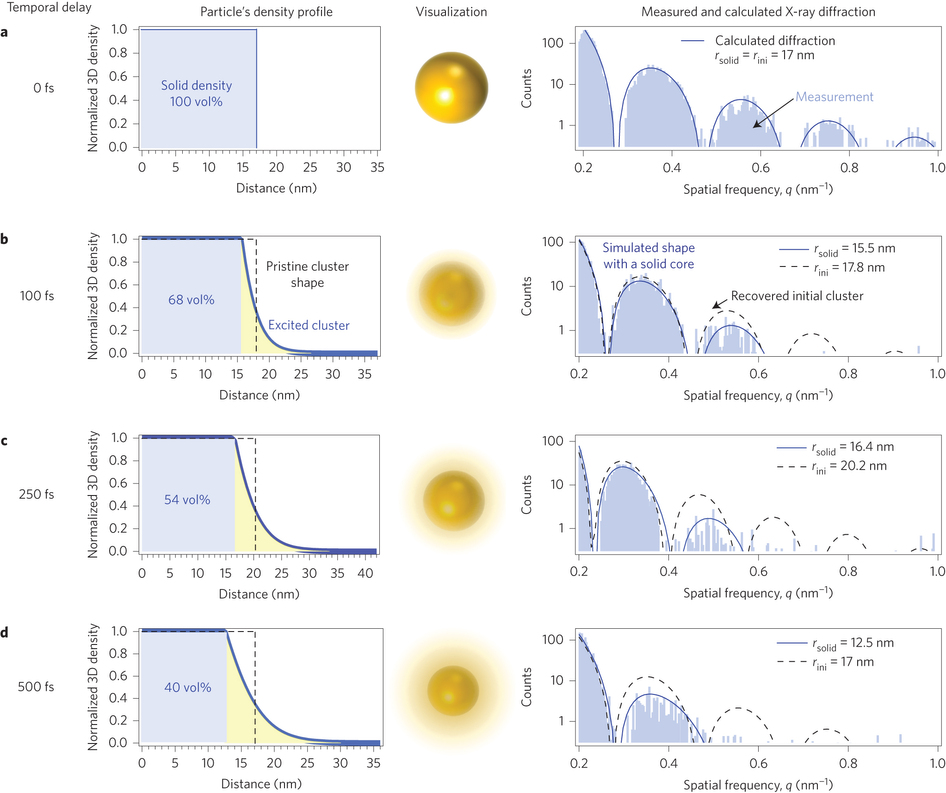
\includegraphics[width=1.00\textwidth]{images/tais-nat-photonics.jpg}
	\caption[Measurement and simulation of the nanoplasma expansion in Xe-clusters.]{Xe-clusters after being pumped with a NIR laser pulse and probed at a certain time delay (indicated left) with a LCLS pulse. Left series, simulation of electron densities. Right series, measured diffraction patterns. The diffraction patterns show a decrease in intensity at larger q values, when the delay is increased. This can be explained through expanding electron densities, i.e., a surface softening. Fourier transformation of electron densities are fitted to the measurement for a solid sphere (dashed line) and an expanding sphere (solid line). From \citep{Gorkhover-2016-NatPho}. Reprinted with permission from Nature Publishing Group.}
	\label{fig:tais-nat-photonics}
\end{figure}
%The nanoplasma transition is so interesting is because every matter irradiated by a free-electron laser will undergo a nanoplasma transition and finally disintegrate. This is a challenge for structural biology and called radiation damage  or sample damage \citep{Neutze-2000-Nature}. Sample damage changes the structure of a biomolecule and it is particularly the structure many scientists want to investigate. In order to prevent falsified measurements, one needs to understand the nanoplasma transition as it occurs while the pulse is propagating through the sample.
The sample damage due to the nanoplasma formation can be divided into two related aspects \cite{Quiney-2010-NatPhys,Curwood-2013-PRA}. One, electronic damage; the electronic configuration of a sample changes inevitably due to photoionization and subsequent processes, which is expected to break bonds and change scattering factors; this limits the ultimately achievable resolution from diffraction imaging. Two, structural damage; the nanoplasma expansion leads to structural changes due to the movement of nuclei \citep{Neutze-2000-Nature}. As these damage aspects are very related, we will refer to them merely as sample- or radiation damage in this thesis. It is currently an active field to investigate these damage processes and determine particularly the timescales of these damage processes, the effect on the measured signal, and the actual structural changes \citep{Bostedt-2012-PRL}. Initial experiments aimed to reveal correlations between diffraction images and ion spectroscopic data using a coincident imaging and spectroscopy technique \citep{Gorkhover-2012-PRL,Rupp-2016-PRL}.\\[1\baselineskip]
%
With the advent of ultrafast pump--probe techniques at XFELs, the nanoplasma expansion could be initiated in a controlled way using the pump-pulse, while the probe-pulse creates a snapshot of the nanoplasma formation and expansion. A first experiment used an infra-red-pump and soft X-ray FEL-probe pulse to study the nanoplasma expansion \citep{Gorkhover-2016-NatPho,Schorb-2012-APL}. Figure \ref{fig:tais-nat-photonics} shows diffraction images of Xe-clusters from this study. The diffraction images have been modeled with Fourier-transformed electron densities. As the time delay, $\Delta t$, between pump- and probe-pulse is varied on the hundred femtoseconds timescale, the diffraction images of the \SIrange{15}{20}{\nano\meter} radius Xe-cluster show declining intensities at larger spatial frequencies, $q$. The loss in signal could be explained through a \textit{surface softening} of the electron density\index{electron density!surface softening} \citep{Hau-Riege-2008-PRE,Peltz-2014-PRL}. This means for the nanoplasma expansion that initially the outer atomic layers of a Xe-cluster expand, and only at longer time delays inner atomic layers begin to expand. It remains a question however, whether the nanoplasma responds similarly to an X-ray induced formation.\\[1\baselineskip]
%In that study, an electron temperature of \SI{\sim 200}{\electronvolt} could be measured by comparing plasma simulations to the ion spectroscopy signal. The spatial resolution of the diffraction patterns has been estimated to be 8 nm, but by assuming a spherical shape of the clusters, the electron density model is sensitive below this resolution.
\begin{figure}
	\centering
		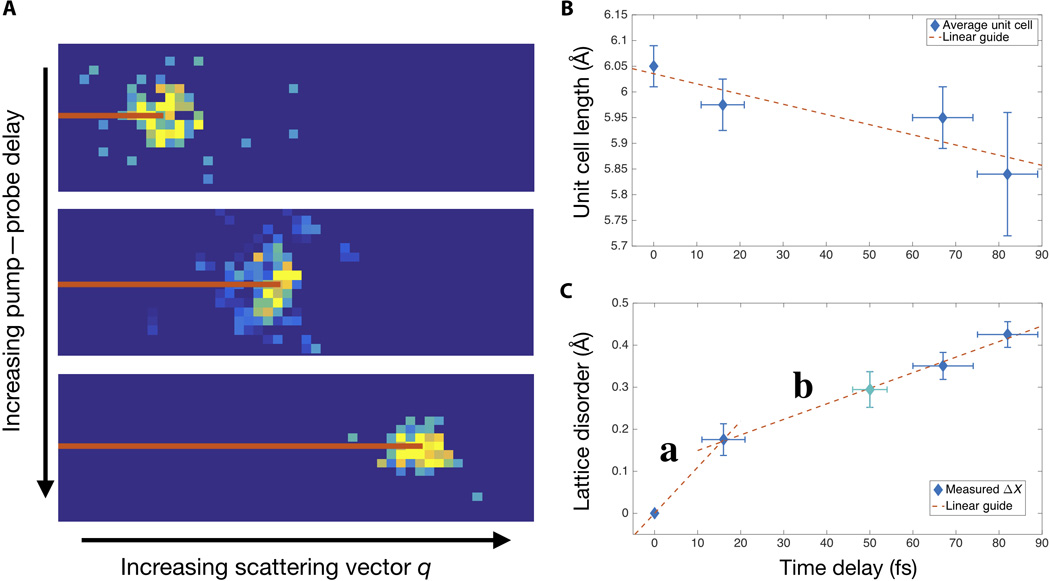
\includegraphics[width=0.80\textwidth]{images/ken-science.jpg}
	\caption[Experiment that shows early evolution of the nanoplasma transition.]{X-ray pump--X-ray probe scattering experiment on Xe-clusters that shows an early evolution of the nanoplasma transition. \textbf{A}, single-shot Bragg peaks at varying time delays. The scattering vector q increases over time delay. \textbf{B}, unit cell length over time delay. The clusters exhibit a \textit{transient lattice compression}. \textbf{C}, Lattice disorder over time delay. The measured fcc lattice is becoming disordered after being pumped with an X-ray pulse. From \citep{Ferguson-2016-SciAdv}. Reprinted with permission from AAAS.}
	\label{fig:ken-science}
\end{figure}
So, an X-ray pump--X-ray probe study at \SI{8.3}{\kilo\electronvolt} using the technique described in Section \ref{sec:twin-bunch-pump-probe} followed at a later time \citep{Ferguson-2016-SciAdv}. Here, a coincident measurement of Bragg powder patterns and ion spectroscopy data was performed and time delays up to $\Delta t<\SI{100}{\femto\second}$ could be observed.
%, xenon clusters compress in size. Since clusters form as a crystal\footnote{See Section \ref{sec:homogenous-cluster}.}, one can determine their structure through crystallographic approaches as it is explained in full detail in \citep[][chapter 5]{Als-Nielson-2011-JWS}
%\footnote{In short, crystals scatter light and create Bragg spots at large $\lvert \vec{Q}\rvert$-values. These Bragg spotts occur when Bragg's law is fulfilled. Bragg's law reads $m \lambda = 2d \sin\left(\frac{\Theta}{2}\right)$,\index{Bragg's law} with $m$ being an integer, $\lambda$ being the wavelength of the scattered light, $d$ the distance between crystalline layers and $\Theta$ the scattering angle. When Bragg's condition is fulfilled, the rays interfere constructively and the location of the Bragg peaks gives insight to the crystalline structure.}. 
%which occur under certain conditions over the scattering vector, $\vec{Q_{\text{peak}}}$. In the figure, the signal moves to larger scattering vectors and, as $\lvert \vec{Q_{\text{peak}}}\rvert=\tfrac{2\pi}{a}$, 
Figure \ref{fig:ken-science}A shows the measured Bragg peaks of Xe-clusters as a function of $\Delta t$. The analyzed signal shows that the unit cell length shrinks over the time delay range $\Delta t =$ \SIrange{0}{80}{\femto\second}, which means that the cluster undergoes a \textit{transient lattice compression} before it begins the nanoplasma expansion. This unintuitive and contradictory result is attributed to the changes in electronic configuration upon ionization. Quasi-free electrons that are trapped in the cluster's Coulomb potential have an increased mobility. These electrons act like delocalized valence electrons that change the cluster's weak van der Waals bonds to a more ``metallic-like'' state. The change in bond character changes the bond length. Due to the limitations in the time delay, it could not be determined, whether the transient lattice compression is followed immediately by a nanoplasma expansion.\\[1\baselineskip]
%As a result, the unit cell changes on the {\AA}ngstrom length scale and the lattice becomes increasingly disordered (see Figure \ref{fig:ken-science}c).
%These two studies allow us to conclude that the nanoplasma transition is a multistep process. First, the initial ionization occurs, followed by an increased Coulomb potential that traps electrons, which then change the structure of the nanosample, e.g., compression of a lattice. Eventually, the system becomes strongly ionized and hot such that Coulomb and hydrodynamic forces start an expansion of the system until the sample disintegrates into its atomic components.
Part of this thesis is to build on and complement the results of the above studies (see Section \ref{sec:xenon-data}). The used X-ray pump--X-ray probe method in this thesis (see Section \ref{sec:k-based-pump--probe}) has similar parameters to current bio-molecule imaging setups such that a nanoplasma formation and expansion can be observed under the conditions of typical single molecule imaging experiments. The pump-pulse has intensities of \SI{\sim 2e16}{\watt\per\square\centi\meter} and the probe-pulse \SI{\sim 2e17}{\watt\per\square\centi\meter}. Here, radiation damage remains a major challenge and is expected to limit maximum achievable resolutions \cite{Aquila-2015-StrucDyn}. Furthermore, the pump--probe method of this thesis experiment allows a time delay range from $\Delta t=$ \SIrange{0}{800}{\femto\second}, thus extending the time delay window of above's X-ray pump--X-ray probe study, and also focuses on the physics of sacrificial layers (see below).
%
%
%
\subsection{Sacrificial layers slow the nanoplasma expansion}\label{sec:tampered-layers}
%%%%%%%%%%%%%%
%- Step by step explanation on the formation of the nanoplasma, pointing out the differences between tampered and pristine clusters
%
%
%
%%%%%%%%%%%%
As we have discussed in the last section, radiation damage occurs as the nanoparticle is exposed to the light pulse, where pulse durations are comparable to Auger decay rates. Thus, the principle of \textit{diffraction before destruction} \citep{Neutze-2000-Nature} demands stringent light source parameters to image a nanoparticle before structural damage, namely X-ray fluences of \SIrange{e13}{e15}{\photons\per\square\micro\meter} and pulse lengths of a few femtoseconds or shorter \citep{Hau-Riege-2005-PRE}. But, these parameters are likely not achievable with the currently planned XFEL light sources \cite{Huldt-2003-JSB}. There have been several proposals to reduce the requirements to light sources \citep{Aquila-2015-StrucDyn} by either reducing or accounting for the effects of radiation damage and here are three promising candidates listed: One, radiation damage effects can - in principle - be accounted for by computer models using, e.g., atomistic cross-section calculations for small biological molecules \cite{Ho-2016-PRA,Quiney-2010-NatPhys,Yoon-2016-scirep}. Two, single particles can be aligned prior to the imaging process \citep{Hau-Riege-2005-PRE} and the known orientation of a reproducible nanoparticle in a 2D projection, i.e., the diffraction image, allows, for example, the averaging of multiple diffraction images; molecule alignment has seen some success for small molecules \citep{Kupper-2014-PRL}, but it is currently unknown, whether this is applicable for larger molecules. The strong light fields that are needed to align the molecules, may change the molecule's structure. Three, nanoparticles or biological molecules can be encapsulated with sacrificial layers \citep{Hau-Riege-2007-PRL}, which slow the progress of the nanoplasma expansion. The tamper supplies the imaged nanoparticle with electrons and the ionized tamper is sacrificed to delay sample damage. This allows longer light pulses to perform the diffractive imaging (see Figure \ref{fig:tamper-layer} and the left panel of \ref{fig:sacrificial-image}). Part of this thesis is to investigate the physics of sacrificial layers, which is why this is discussed in more detail below.\\[1\baselineskip]
%
Initially water has been proposed as tamper layer material for biological particles \citep{Hau-Riege-2007-PRL}, but recent discussions \citep{Aquila-2015-StrucDyn} suggest that water tamper layers tend to become uneven in thicker layers. The tamper layers are usually not uniform around the sample due to a mix of hydrophobic and hydrophilic surfaces on typical biological particles. It is important to have a uniform and thin tamper layer to cope with the contributions from the layer to the diffraction image. These contributions can be reduced by averaging multiple diffraction patterns and removing the average contributions from the layer \citep{Hau-Riege-2007-PRL,Maia-2009-PRE}. For the averaging of the diffraction images, the orientation of the nanoparticle needs to be accounted. Tamper layers have been used at FLASH\footnote{Short for \textbf{F}ree electron \textbf{LAS}er in \textbf{H}amburg. An XUV free electron laser in Hamburg, Germany.}\index{Free electron LASer in Hamburg!FLASH} using fixed targets that were mounted on a stage as a sample \citep{Hau-Riege-2010-PRL}. Here, a silicon tamper layer was placed around an aluminum pillar and compared to an aluminum pillar without a tamper layer (see Figure \ref{fig:tamper-layer}). The effects of the sacrificial layers were immediately obvious and the tamper ensured the sample integrity over a period of at least \SI{5}{\pico\second} after the irradiation with a \SI{25}{\femto\second}-long \SI{13.5}{\nano\meter} FLASH pulse.\\[1\baselineskip]
%
\begin{figure}
	\centering
		a)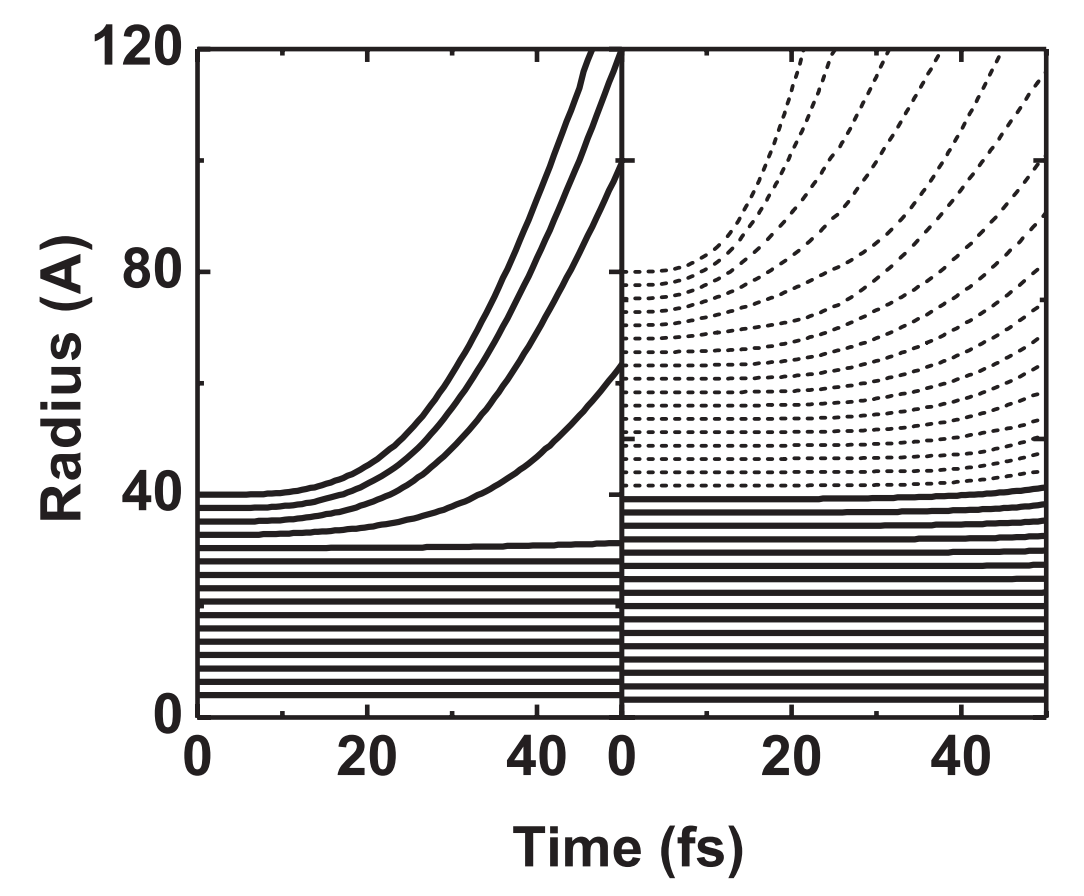
\includegraphics[width=0.49\textwidth]{images/tamper-layers.png}
		b)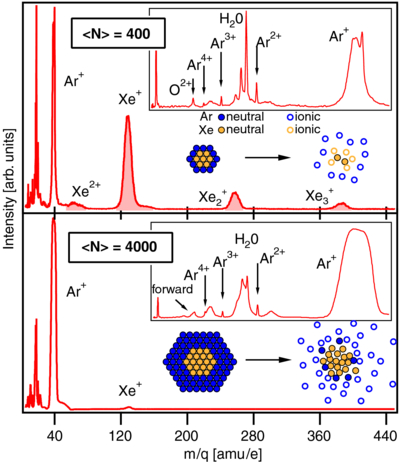
\includegraphics[width=0.4\textwidth]{images/Hoener-image.jpg}
	\caption[Tamper layers and nanoparticles that undergo a nanoplasma formation.]{a) Simulations of atomic layers of a nanoparticle that undergoes a nanoplasma formation without tamper layers (left) and with tamper layers (right, tamper dashed line). From \citep{Hau-Riege-2007-PRL}. Reprinted with permission from APS. b) TOF traces of ArXe-cluster of different sizes, $\left\langle N\right\rangle$. Insets show m/q < 40. From \citep[\href{https://creativecommons.org/licenses/by/3.0/}{\ccby}]{Hoener-2008-JPB}.}
	\label{fig:sacrificial-image}
\end{figure}
%
Another study \citep{Hoener-2008-JPB} that is very close to the idea of tamper layers and the work described in this thesis is shown in the right panel of Figure \ref{fig:sacrificial-image}. Here pristine Ar- and Xe- clusters as well as heterogeneous ArXe-clusters were investigated. The two rare-gases form a \textit{core--shell system}, whereby the cluster's core consists of Xe-atoms and the shell is build of Ar-atoms. The clusters were irradiated with \SI{93}{\electronvolt} photons from FLASH to undergo a nanoplasma formation and expansion. At this photon energy, dominantly xenon atoms are ionized. Figure \ref{fig:sacrificial-image}b) shows time-of-flight (TOF) mass spectra that are explained in more detail in Section \ref{sec:TOF-spectrometer}. The top panel of Figure \ref{fig:sacrificial-image}b) shows TOF traces of small ArXe-clusters with $\left\langle N\right\rangle = 400$, where mostly Ar- and Xe-ions are measured. The bottom panel of Figure \ref{fig:sacrificial-image}b) shows TOF traces of larger ArXe-clusters with $\left\langle N\right\rangle = 4000$, where the Xe-ion count is significantly reduced. The data also indicates that argon atoms in the large cluster case release more kinetic energy than in the small cluster case.
%The experiment reveals that in smaller core--shell systems of ArXe-clusters with \num{400} particles (Figure \ref{fig:sacrificial-image} top-right panel) the time-of-flight (TOF) mass spectroscopy\index{time-of-flight!mass spectroscopy} (see Section \ref{sec:TOF-spectrometer}) data show Xe- and Ar-ions, while in larger core--shell systems of ArXe-clusters with \num{4000} particles (Figure \ref{fig:sacrificial-image} bottom-right panel) dominantly Ar-ions can be found in the TOF data. 
As we have discussed in Section \ref{sec:nanoplasma-expansion}, larger clusters trap electrons efficiently in their deep Coulomb potential. These trapped electrons are available for recombination \cite{Hoener-2008-JPB,Fennel-2010-RMP} with other ionized atoms in the cluster. This is what the large ArXe-clusters TOF data indicates, here Xe-ions recombine with electrons that were attracted to the center of the core--shell system due to the deep Coulomb potential. Neutral xenon atoms are not detected by the TOF detector. The Ar-atoms in the outer shell are therefore \textit{charge-transfer ionized} and this tamper layer is then shed off (sacrificed) by the mixed ArXe-cluster.\\[1\baselineskip]
%
These are promising results that sacrificial layers slow the nanoplasma formation and expansion of nanoparticles that are exposed to highly intense X-ray pulses. While the underlying processes of a tamper layer are more and more understood and its application for diffractive imaging is demanded \cite{Aquila-2015-StrucDyn}, experiments have not jet produced data that comes close to the conditions of typical diffractive imaging setups at XFELs. Here nanoparticles are typically injected using gas or aerosol jets to take diffraction images at high rates. The sample injection then poses the question, which tamper material should be used and how it can be placed reproducibly around a nanoparticle?\\[1\baselineskip]
%
Helium droplets have a long tradition for studies of embedded species due to the unique attributes of the quantum fluid \citep{VonHaeften-1997-PRL,VonPietrowski-2006-EPJ,Stienkemeier-2006-JPhysB,Buchta-2013-JCPA,Gomez-2014-Science}. About a decade ago, heterogeneous HeXe-clusters were studied theoretically as a core--shell system \citep{Mikaberidze-2008-PRA} and it was proposed to use helium tamper layers to slow and reduce the effects of a nanoplasma formation and expansion upon irradiation with an XFEL.\\[1\baselineskip]
%
This thesis investigates HeXe-clusters experimentally using the previously mentioned X-ray multipulse operations at LCLS (see Section \ref{sec:novel-pump--probe-tech}) and a coincident measurement of diffraction images and TOF mass spectra (see Chapter \ref{ch:exp_setup}. The data is analyzed using, for example, iterative phase-retrieval algorithms that reveal the first real-space reconstructions of rare-gas clusters (see Chapter \ref{ch:methods}). We find evidence in HeXe-clusters that the He-shell acts as a sacrificial layer, which is discussed further in Chapter \ref{ch:results}.
%Another way is to fundamentally increase resolution in single particle imaging due to prior alignment of particles such that their orientation is known while the image is taken. 
%As we have discussed, the nanoplasma formation occurs on the femtosecond timescale and affects diffraction patterns. To \textit{outrun} this radiation damage, pulses from the XFEL must be shorter than the lifetime of Auger processes, thus a few femtoseconds long. And by limiting the XFEL pulse duration, one limits the pulse energy\index{pulse energy} as current bunch compression methods typically generate much less fluence. Often, this fluence is not enough and means that many coherent diffractive imaging experiments are currently performed with pulse widths of 40 fs or more to generate enough scattered intensity. But even if these technical limitations can be overcome, outrunning radiation damage does not circumvent photoionization and it is therefore expected that few-femtoseconds long pulses have spatial resolution limitations \citep{Aquila-2015-StrucDyn}. To be more precise, it is an open question, whether electron densities and particular bonding configuration are obtainable by solely outrunning radiation damage. Although radiation damage is unavoidable it can be mitigated in several ways. 
%One way to mitigate radiation damage is to simulate the effects, however, this can only be done for small particles. 
%Here, it should be noted that recent advances with diffractive imaging algorithms made it possible to computationally determine the orientation of a particle at the time of imaging \citep{Loh-2009-PRE,Ekeberg-2015-PRL}. The orientation can be aromatically determined -- without prior knowledge -- when at least a few hundred diffraction images are provided. However, in this thesis, we shall discuss a method to reduce the effects of radiation damage through artificial tamper layers. Artificial shells around a sample supply it with electrons and function as a sacrificial layer that protects the sample \citep{Hau-Riege-2010-PRL}. For aerosol particles, this method has only been investigated through ion spectroscopy \citep{Hoener-2008-JPB,Ziemkewitz-2017-unpublished}.\\[1\baselineskip]
%
%
%
%
%